\chapter{Exploratory anodes studies with DEIS}
\label{chap:anodes}

Dynamic impedance spectroscopy measurements have demonstrated a strong correlation of the instantaneous impedance with state of charge and state of health in commercial lithium-ion batteries, as established in chapter \ref{chap:coins}.  
In chapters \ref{chap:LTP} and \ref{chap:capacitor}, three-electrode flooded  and compact cells were used to isolate the impedance of individual electrodes and to relate the time-varying spectra to physically meaningful parameters.  
These results motivate the extension of dynamic impedance spectroscopy to batteries in three-electrode configuration with the aim of isolate and identify degradation phenomena under operating conditions.
  
This chapter focuses on negative battery electrodes for lithium and sodium intercalation because, compared to positive electrodes, they are commonly associated with the onset of the most critical degradation mechanisms.  
Two processes are of particular technological relevance:
\begin{enumerate}
    \item \textbf{Metal plating} (lithium or sodium), which becomes especially problematic during high-rate charging and is associated with rapid loss of active lithium/sodium and possible cell failure.
    \item \textbf{Growth and restructuring of the solid electrolyte interphase (SEI)}, which increases interfacial resistance and affects rate capability.
\end{enumerate}

Both phenomena alter the local electrochemical kinetics and therefore should manifest distinct signatures in the time-resolved impedance.  

To resolve the potential of the single electrodes, a micro-reference electrode can be used in compact cell \cite{raccichiniCriticalReviewReference2019}, the typical format of battery cells.
Unlike in flooded cells, the restricted volume and stack pressure limit the size and placement of reference electrodes, and improper positioning can lead to significant measurement artifacts, as demonstrated in chapter~\ref{chap:LTP}.  
For this reason, microscopic metal wires with localized exposed tips were used as reference electrodes and placed directly between the separators, enabling a closer approximation of a point-like reference potential inside the stack.

% The experiments presented in this chapter are exploratory in nature.  
% The fabrication of micro-reference electrodes proved challenging, and the reproducibility across cells was limited.  
% Despite these constraints, the measurements reveal several qualitative trends that are scientifically valuable and motivate further targeted investigations.

This chapter discusses DEIS measurements performed on three different half-cell configurations:
\begin{itemize}
    \item graphite vs.\ lithium, using electrodeposited lithium on insulated copper wire as the reference electrode;
    \item SiCN(O) vs.\ sodium, using electrodeposited sodium on insulated copper wire as the reference electrode (two independent assemblies);
    \item sodium vs.\ sodium, using electrodeposited sodium on insulated copper wire as the reference electrode.
\end{itemize}

The overarching research question guiding this work is:
Can dynamic impedance spectroscopy identify transient interfacial processes such as SEI formation, staging phenomena, or metal plating directly during electrode operation?

The following sections present the materials, cell designs, DEIS parameters, and qualitative analysis of the impedance behavior for each electrode type.

\section{Experimentals}

\subsection{Active materials}

\subsubsection{Graphite}

Graphite is the standard negative electrode material in commercial lithium-ion batteries, owing to its reversible Li\textsuperscript{+} intercalation, good rate capability, and long-term cyclability.  
Its staging transitions, solid-electrolyte interphase (SEI) formation, and susceptibility to lithium plating under high-rate charging make it an ideal system for testing whether DEIS can resolve transient interfacial phenomena \emph{in situ}.

In this work, graphite half-cells in pouch format were assembled to investigate three aspects:
\begin{enumerate}
    \item the evolution of impedance during different intercalation stages;
    \item the onset of plating-like signatures during high-current reduction;
    \item the asymmetry between reduction and oxidation kinetics under non-stationary conditions.
\end{enumerate}
These measurements serve as a reference point because the electrochemistry of graphite is well established and provides a benchmark against which to interpret more complex materials such as SiCN(O).

\subsubsection{SiCN(O)}

Silicon carbonitride SiCN(O) is a polymer-derived ceramic with a tunable disordered network composed of Si-N, Si-C, and C-C bonding motifs.  
Depending on the precursor and pyrolysis conditions, the material exhibits high microporosity, moderate electronic conductivity, and good chemical stability in non-aqueous electrolytes.  
These characteristics make SiCN(O) a promising negative electrode material for sodium-ion batteries, where hard carbon is currently the state of the art \cite{liuReviewHardCarbon2025}.

In contrast to graphite, SiCN(O) does not undergo intercalation into well-defined crystallographic positions.  
Instead, several storage mechanisms have been proposed in the literature—including surface adsorption, pore filling, and reversible metal deposition within the nanoporosity \cite{liuReviewHardCarbon2025}.  
The relative contributions of these processes remain under debate.

The electrodes containing SiCN(O) as active materials were prepared by Dr.-Ing. Marco Melzi d'Eril within a collaboration with the Technical University of Darmstadt.
A detailed discussion of the chemistry, synthesis routes, and structural characterization of SiCN(O) is provided in Appendix~\ref{app:SiCNO_background}.  
Here, we focus solely on the motivation for DEIS measurements.

Two properties of SiCN(O) make it particularly interesting for dynamic impedance studies:
\begin{enumerate}
    \item its highly porous microstructure, which can host different Na storage modes that may evolve during cycling;
    \item experimental evidence from galvanostatic cycling \cite{derilReversibleSodiumPlating2023} suggesting that lowering the cutoff potential below~0~V vs.\ Na\textsuperscript{+}/Na triggers additional reversible capacity, possibly associated with sodium metal deposition within the pore network.
\end{enumerate}

DEIS offers a unique opportunity to probe whether these mechanisms leave distinct, time-localized signatures in the impedance, especially during the transition between adsorption, insertion-like processes, and hypothesized metal deposition.  
This approach complements conventional characterization methods such as ex situ NMR or Raman spectroscopy by enabling operando tracking of interfacial kinetics.

\subsubsection{Micro-reference electrodes}

Introducing a reference electrode into a pouch-cell configuration presents significant geometric and electrochemical challenges.  
As discussed in chapter~\ref{chap:LTP}, the placement and size of the reference electrode strongly influence the measured impedance, particularly in compact cells where the electric field is highly non-uniform.  
Macroscopic reference electrodes, such as Ag/AgCl or metal strips, distort the potential distribution and introduce artefacts in the high- and mid-frequency regions, making them unsuitable for dynamic impedance measurements in multilayer or small-area cells.

The electrostatic distortion introduced by extended reference electrodes in compact geometries is schematically illustrated in Figure \ref{fig:micro reference positioning}

\begin{figure}[!h]
    \centering
    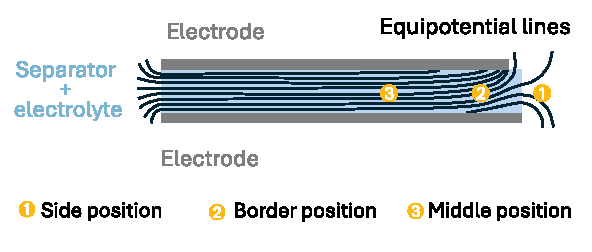
\includegraphics[width = 0.7\textwidth]{figures/anodes/reference electrode position.pdf}
    \caption{Electric field distortion at the electrodes border in compact cells.
    Schematic illustration showing how macroscopic reference electrodes perturb current and potential distribution near the electrode stack, motivating the use of point-like micro-reference electrodes in pouch-cell DEIS.}
    \label{fig:micro reference positioning}
\end{figure}

For this reason, I adopted microscopic reference electrodes based on insulated metal wires with only the cross-section area exposed to the electrolyte.  
Such electrodes approximate a point-like probe and minimize perturbation of the current distribution.  
When placed between two separators at the mid-plane of the stack, they provide an acceptable compromise between electrochemical stability and geometric neutrality.
An illustration of micro-reference electrode integrated into a three-electrode pouch cell is shown in Figure \ref{fig: micro reference pouch}

\begin{figure}[!h]
    \centering
    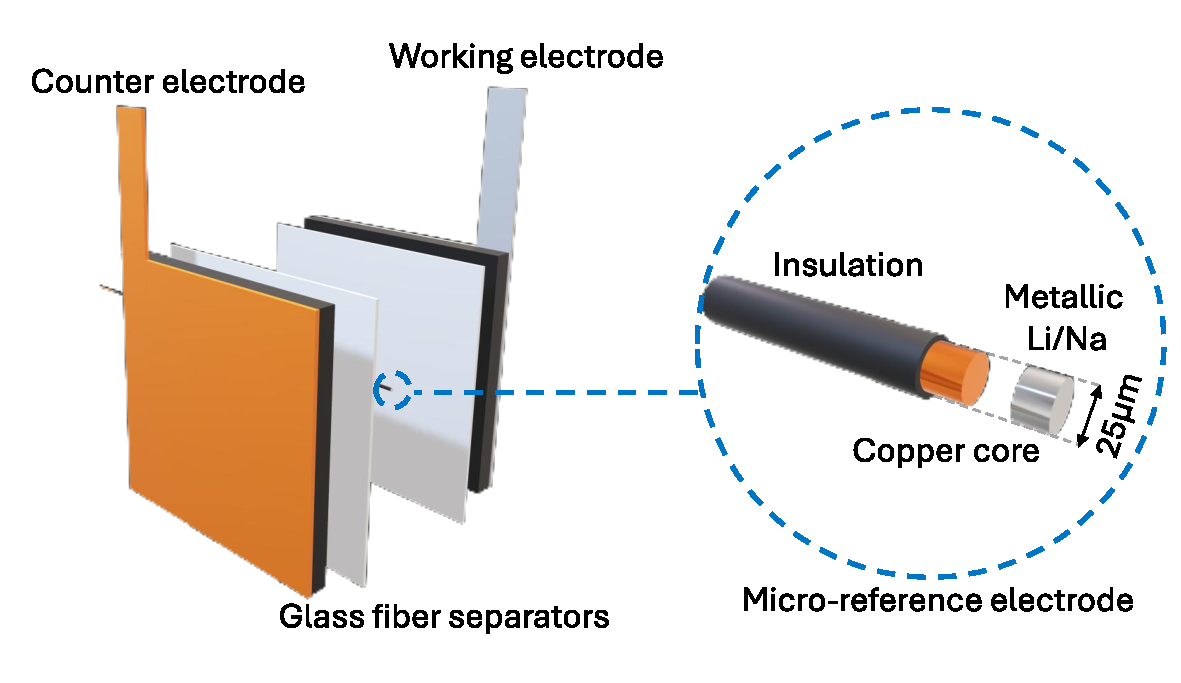
\includegraphics[width = 0.8\textwidth]{figures/anodes/micro reference electrode.pdf}
    \caption{Microscopic reference electrode implemented in a pouch-cell stack.
    Insulated metal wire with only the cross-sectional tip exposed to the electrolyte, positioned between separators to approximate a point-like reference potential while minimizing current-path distortion.}
    \label{fig: micro reference pouch}
\end{figure}

In lithium systems, micro-reference electrodes are achieved by in situ alloying of gold (in the form of wire) and lithium, whereas in sodium systems few attempts were made because its incapacity to alloy with gold \cite{Oehler_2023,solchenbachGoldMicroReferenceElectrode2016, houLithiumGoldReferenceElectrode2020, behlingFormationLithiatedGold2021}. 
Sodium alloys instead with Tin but in a more complex multiphase chemistry \cite{linsenmannReferenceElectrodeSitu2019a}.

In this exploratory work, I could not replicate the lithium-gold alloying procedure found in the literature so I decided to proceed with electrodeposition on copper wires for both lithium and sodium. 
The electrochemical stability of these microscopic electrodes is strongly dependent on the quality of the insulation and the suppression of parasitic side reactions.  
Although the approach enabled DEIS measurements for extended periods, reproducibility remained limited because small imperfections in insulation, wire geometry, or deposition uniformity lead to drifts of the reference potential.

A detailed account of the fabrication procedures, attempts with different substrates, stability tests, and failure modes is provided in Appendix \ref{app:microRE}.  
In this chapter, only the essential aspects are reported, as the purpose of these measurements is not to optimize reference electrode design but to demonstrate that DEIS can be performed operando in three-electrode pouch cells.

To verify the stability of the reference electrode during the measurement, I recorded the OCV between the reference electrode and the metallic counter electrode of the cells.
The voltage difference was always of 1-2 mV at the end of the experiments and even after days or weeks (cell disconnect from the isntrument).

\subsection{Electrode preparation and cell assembling}

\subsubsection{Graphite electrode}
Graphite negative electrodes were prepared from an aqueous slurry containing AF-261 graphite powder, 6\,wt\% Super~P C60 to enhance electronic conductivity, and 3\,wt\% carboxymethylcellulose (CMC) as binder.  
The slurry was cast onto copper foil using an automated doctor-blade coater and dried under vacuum at 80\,$^\circ$C overnight.  
Electrodes were then punched into 2\,cm~$\times$~2\,cm squares and stored in an argon atmosphere prior to cell assembly.

\subsubsection{SiCN(O) electrode}
The SiCN(O) electrodes were obtained from SiCN(O) powder (average particle size $\sim$40\,\textmu m) mixed with 2\,wt\% carbon black to increase electronic conductivity, and a binder system composed of 2\,wt\% CMC and 2\,wt\% styrene-butadiene rubber (SBR).  
The resulting aqueous slurry was cast onto aluminium foil, dried under vacuum at 80\,$^\circ$C for 24\,h, and subsequently punched into 12\,mm diameter disks.  
The synthesis route of SiCN(O), along with bulk characterization data and electrode formulation, is described in detail in Reference \cite{derilReversibleSodiumPlating2023} and is not repeated here.

\subsubsection{Metallic sodium}
Metallic sodium counter electrodes were prepared from commercial sodium-aluminium laminate disks (12\,mm diameter).  
These disks are supplied with protective polymer films on both sides to prevent oxidation and preserve the flatness of the active surface.  
Prior to assembly, the protective foils were removed inside the glovebox and the disks were immediately transferred to the cell stack.

\subsubsection{Electrolytes}
Two electrolytes were used depending on the chemistry:
\begin{itemize}
    \item 1\,M LiPF\textsubscript{6} in EC:DEC (1:1\,w/w) with 2\,wt\% vinyl carbonate (VC) for graphite/Li half-cells;
    \item 1\,M NaPF\textsubscript{6} in EC:DEC (1:1\,w/w) for SiCN(O)/Na and Na/Na cells.
\end{itemize}
All electrolytes were handled in an argon-filled glovebox ($< 0.1$\,ppm O\textsubscript{2}, $< 0.1$\,ppm H\textsubscript{2}O).

\subsubsection{Three-electrode pouch cell}

To assemble these cells, I chose the pouch cell format because it offers a high degree of geometric flexibility, larger electrode areas, and ease of assemble, characteristics that make them a standard platform for laboratory-scale battery development.  
The three-electrode pouch cells were assembled using two layers of glass fiber separator with the micro-reference electrode positioned between them.  
% The design follows the considerations developed in Chapter~\ref{chap:capacitor} and in the literature, which show that positioning the reference at the mid-plane minimizes artifacts in the impedance measurements.  
% This geometry requires a microscopic reference electrode; macroscopic metal-strip references are significantly easier to assemble but introduce impedance artefacts due to their extended surface area and non-uniform potential distribution.

The integration of the micro-reference electrode in graphite/Li pouch cells is shown in Figure \ref{fig:graphite_pouch} and SiCN(O)/Na cells in Figure \ref{fig:SiCNO_pouch}.  
In both cases the current-collector tabs were put in contact to aluminium or nickel leads without welding or other adhesives, and the stack was enclosed in a laminated pouch and sealed under reduced pressure. 

\begin{figure}[!h]
    \centering
    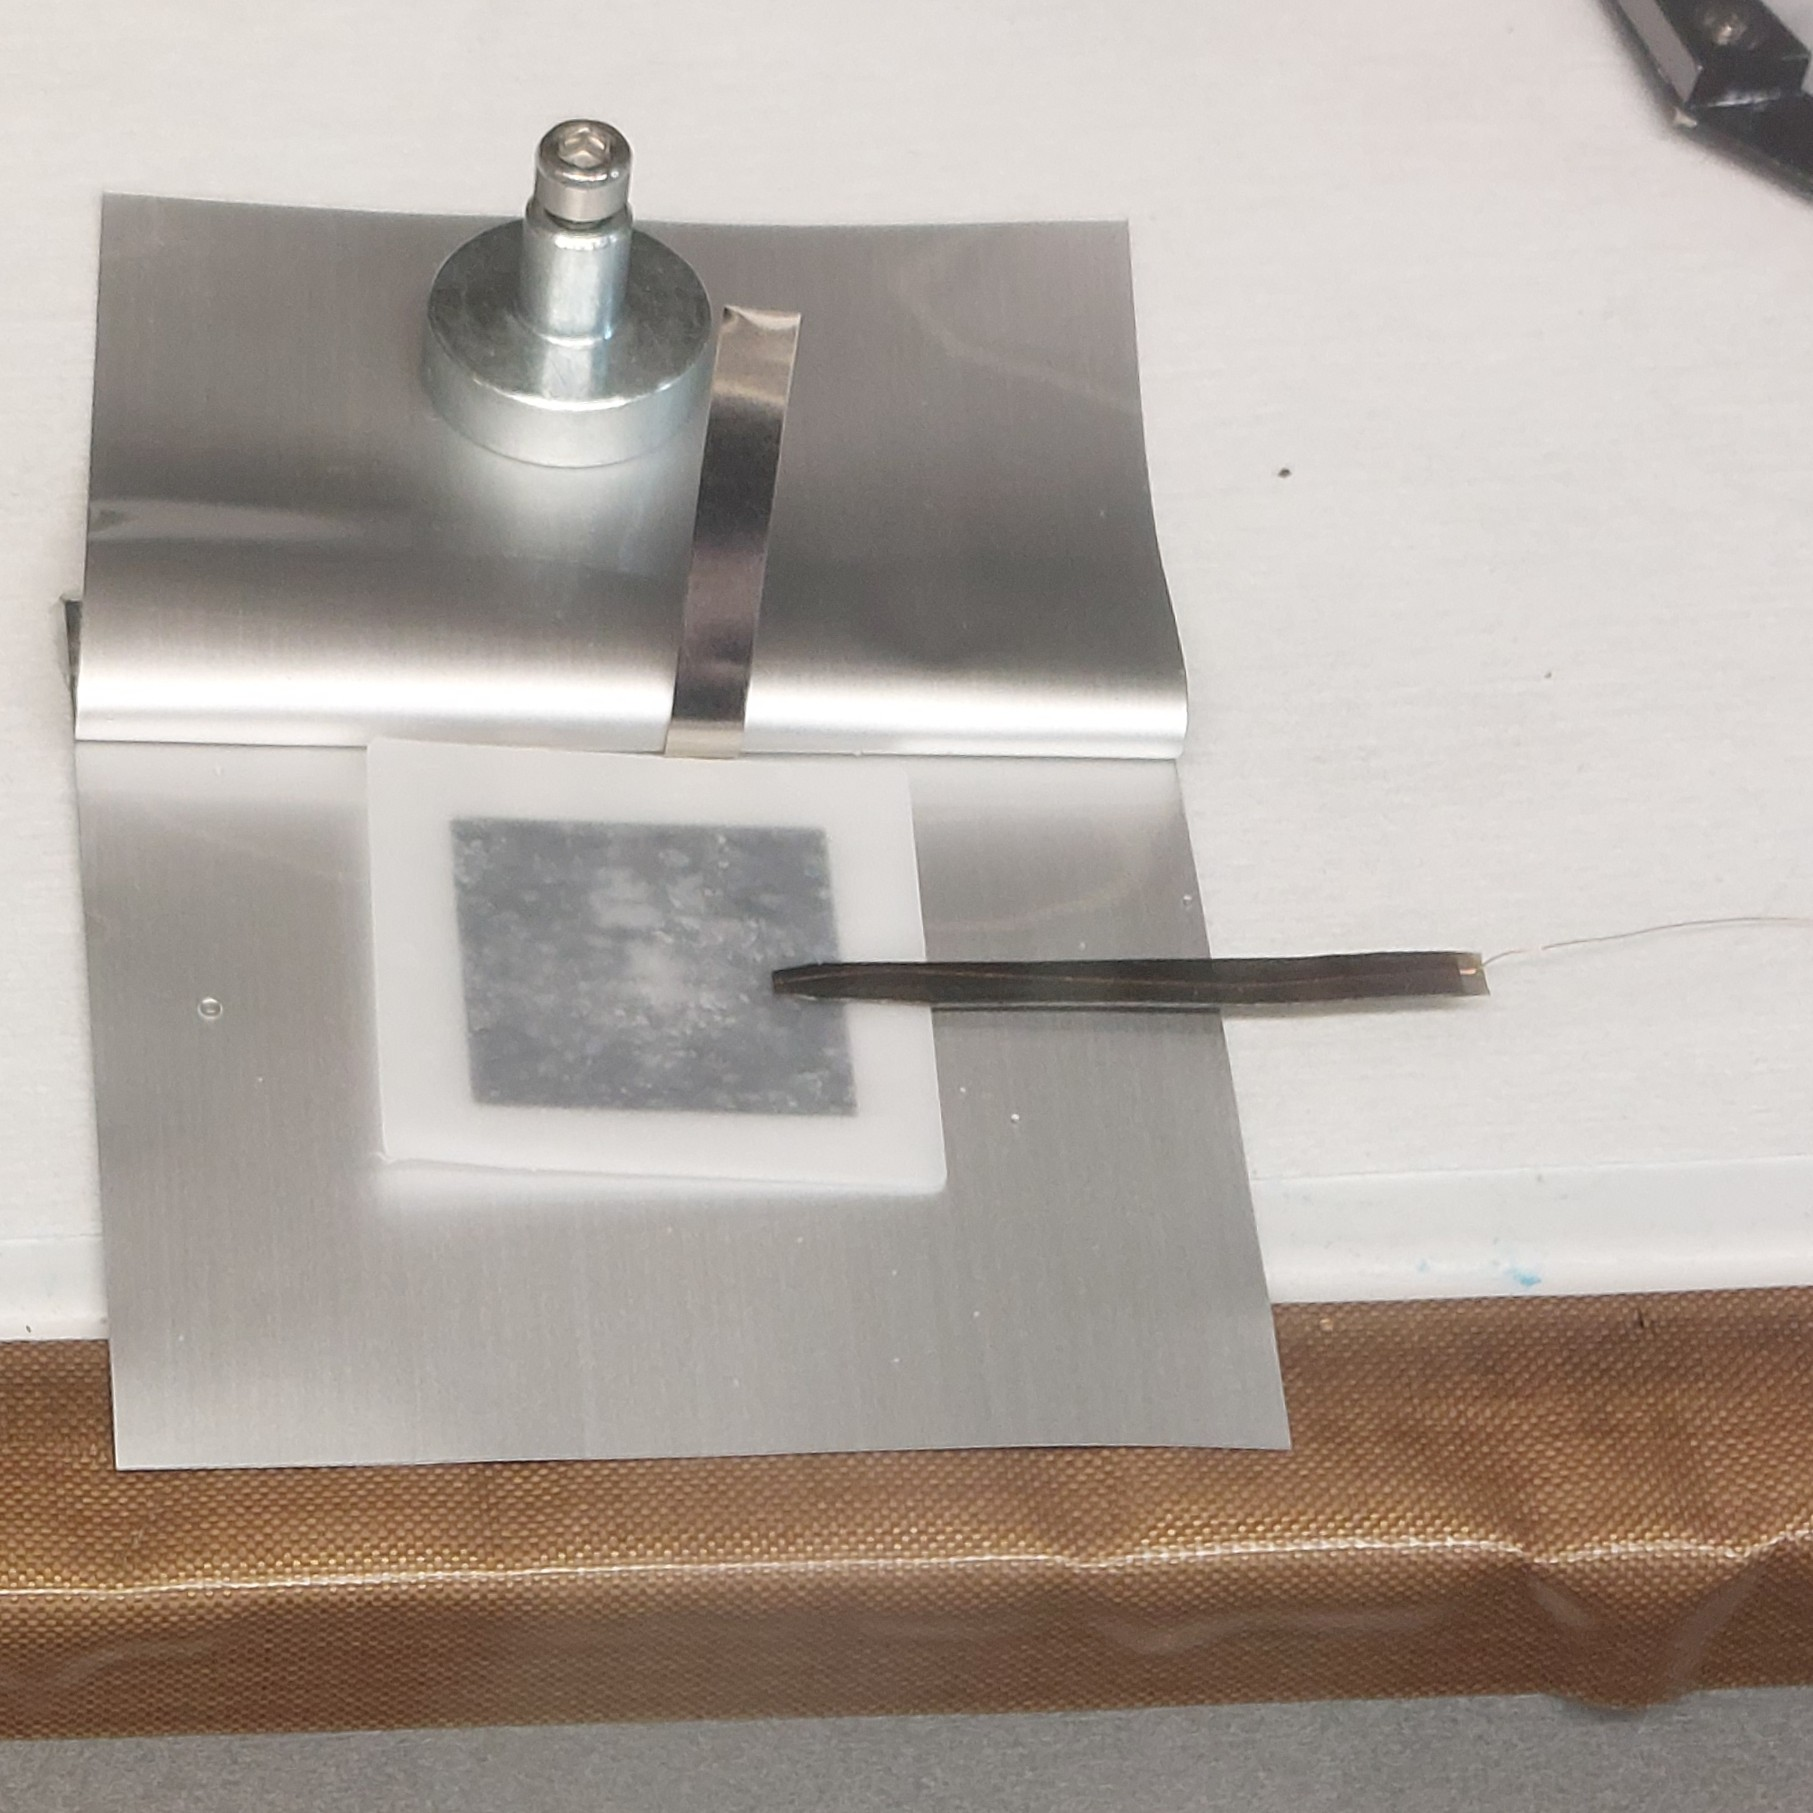
\includegraphics[width=0.45\textwidth]{figures/anodes/graphite_reference_placing.jpg}
    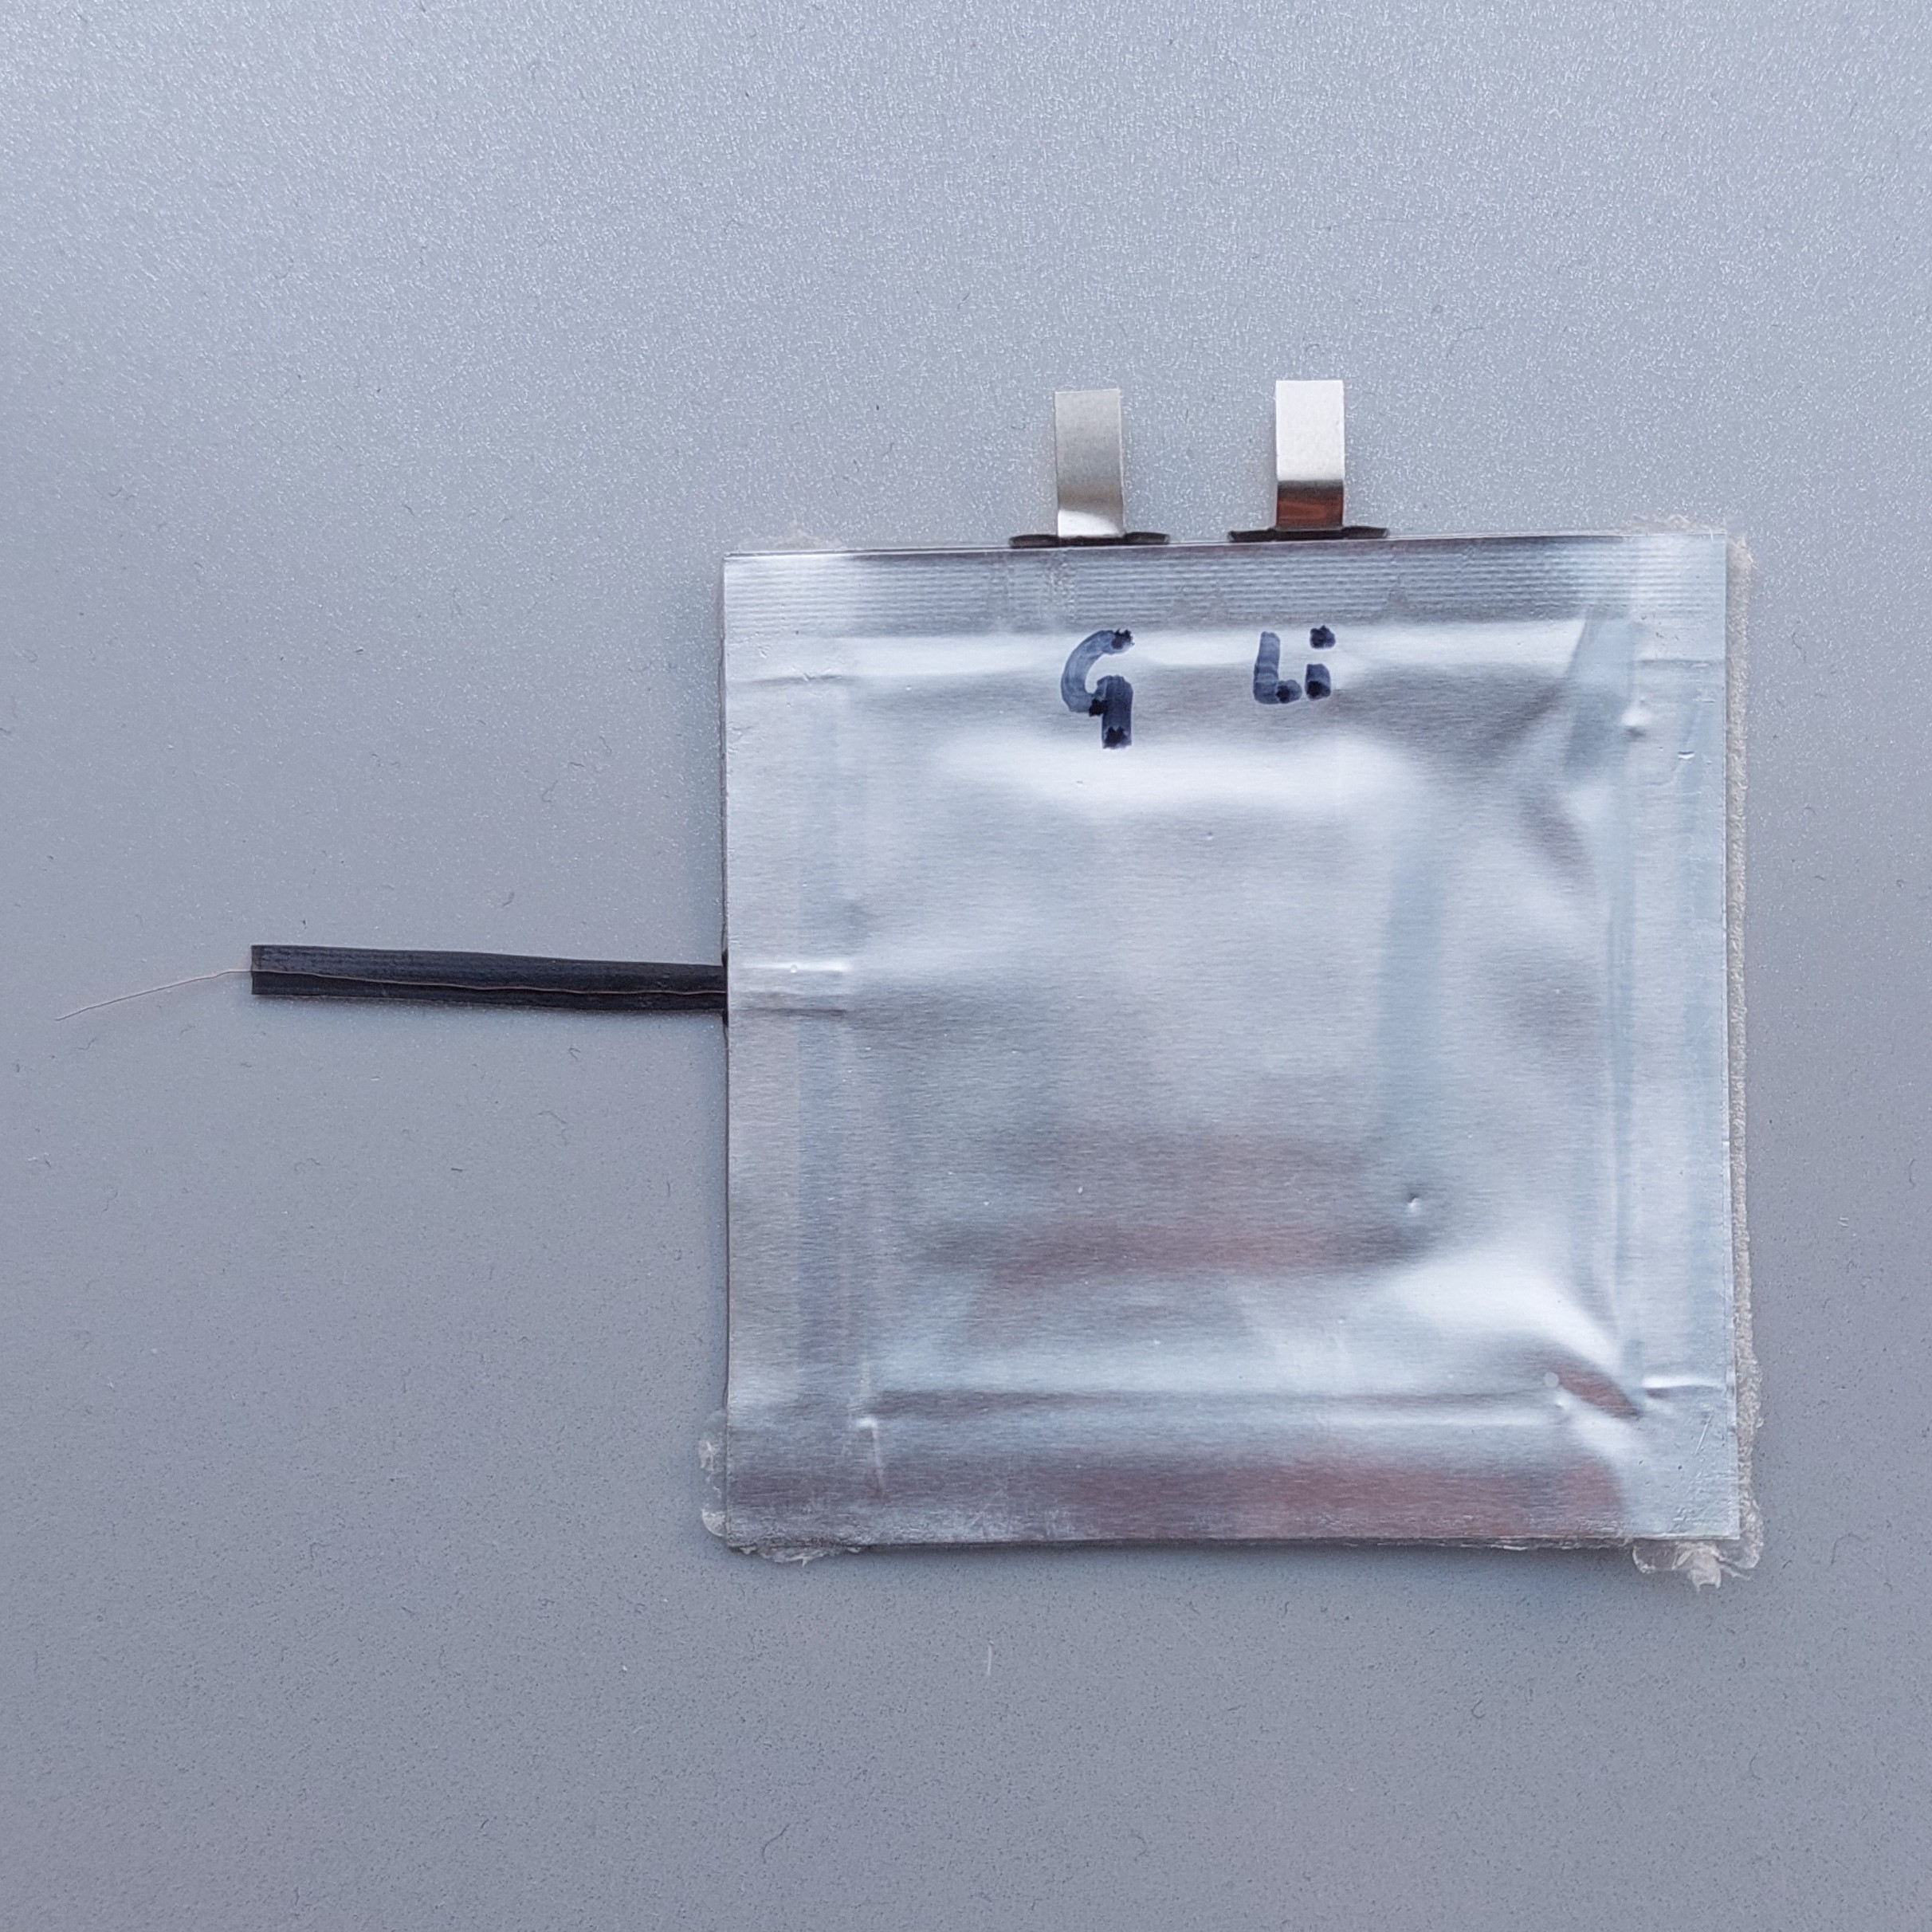
\includegraphics[width=0.45\textwidth]{figures/anodes/graphite_final_pouch_3e.jpg}
    \caption{Three-electrode graphite/Li pouch cell with micro-reference electrode.
    Left: placement of the insulated micro-reference electrode between separators; right: sealed three-electrode pouch cell used for DEIS measurements on graphite half-cells.}
    \label{fig:graphite_pouch}
\end{figure}

\begin{figure}[!h]
    \centering
    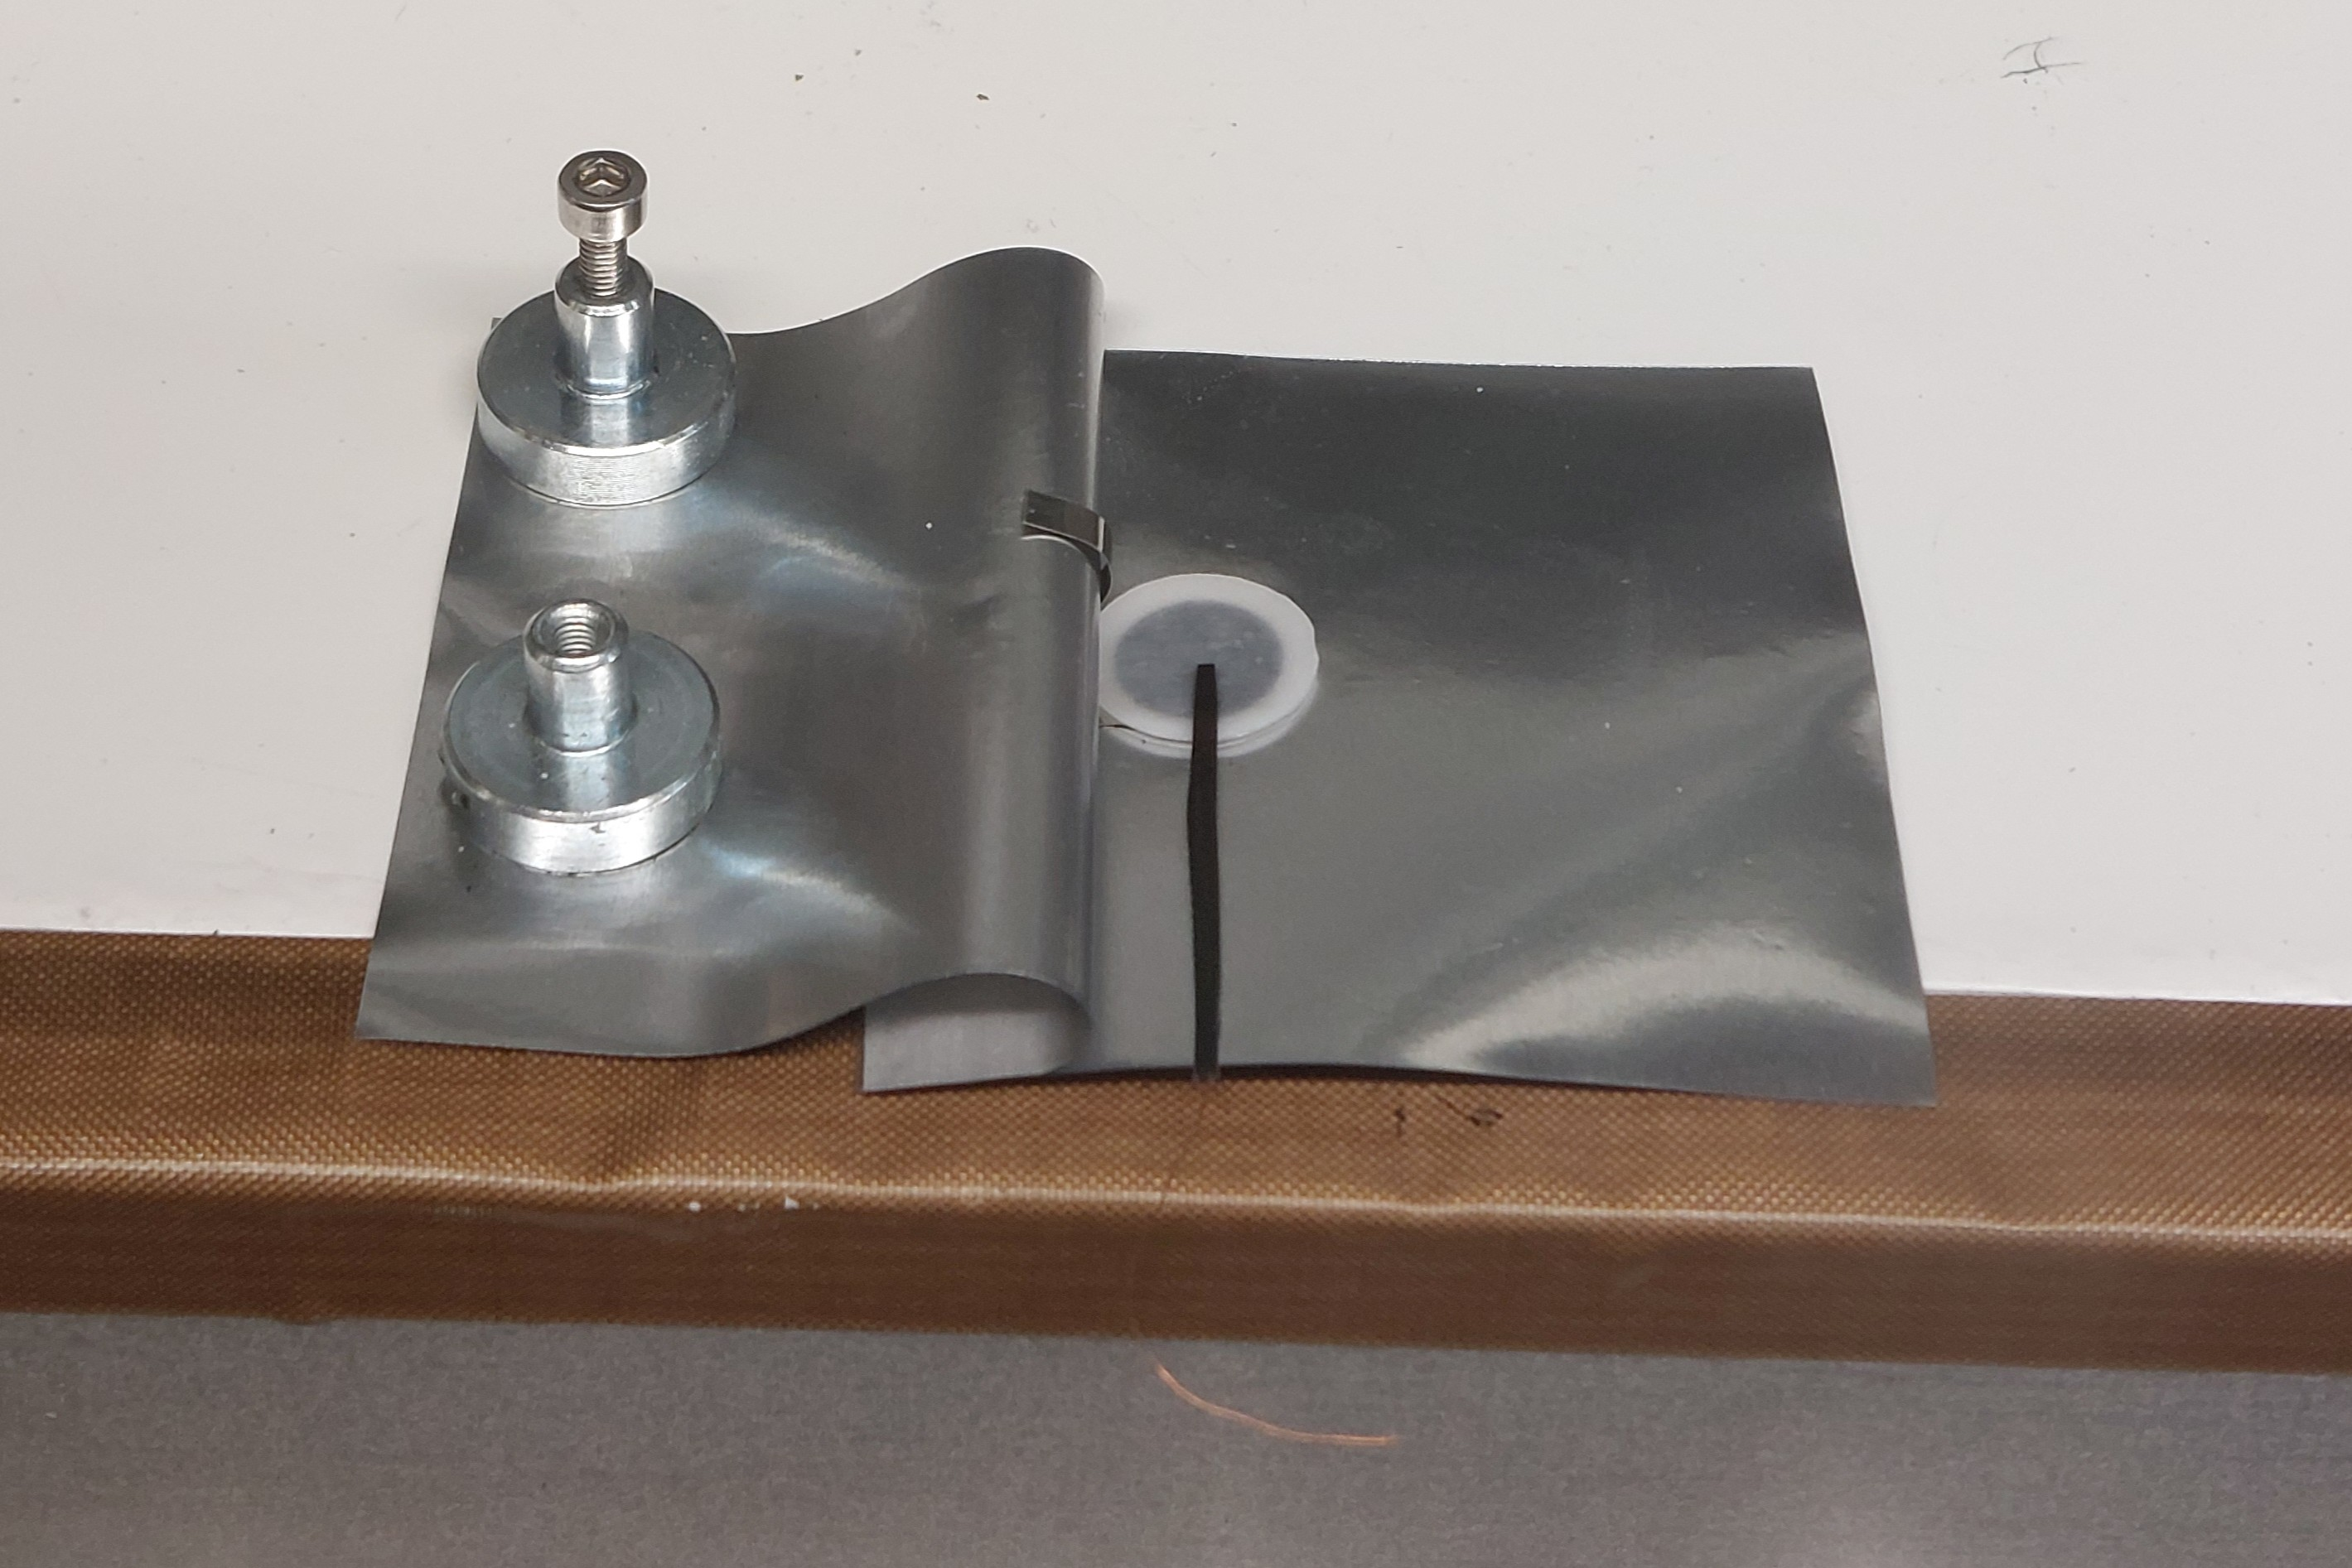
\includegraphics[width=0.57\textwidth]{figures/anodes/SiCN_reference_placing.jpg}
    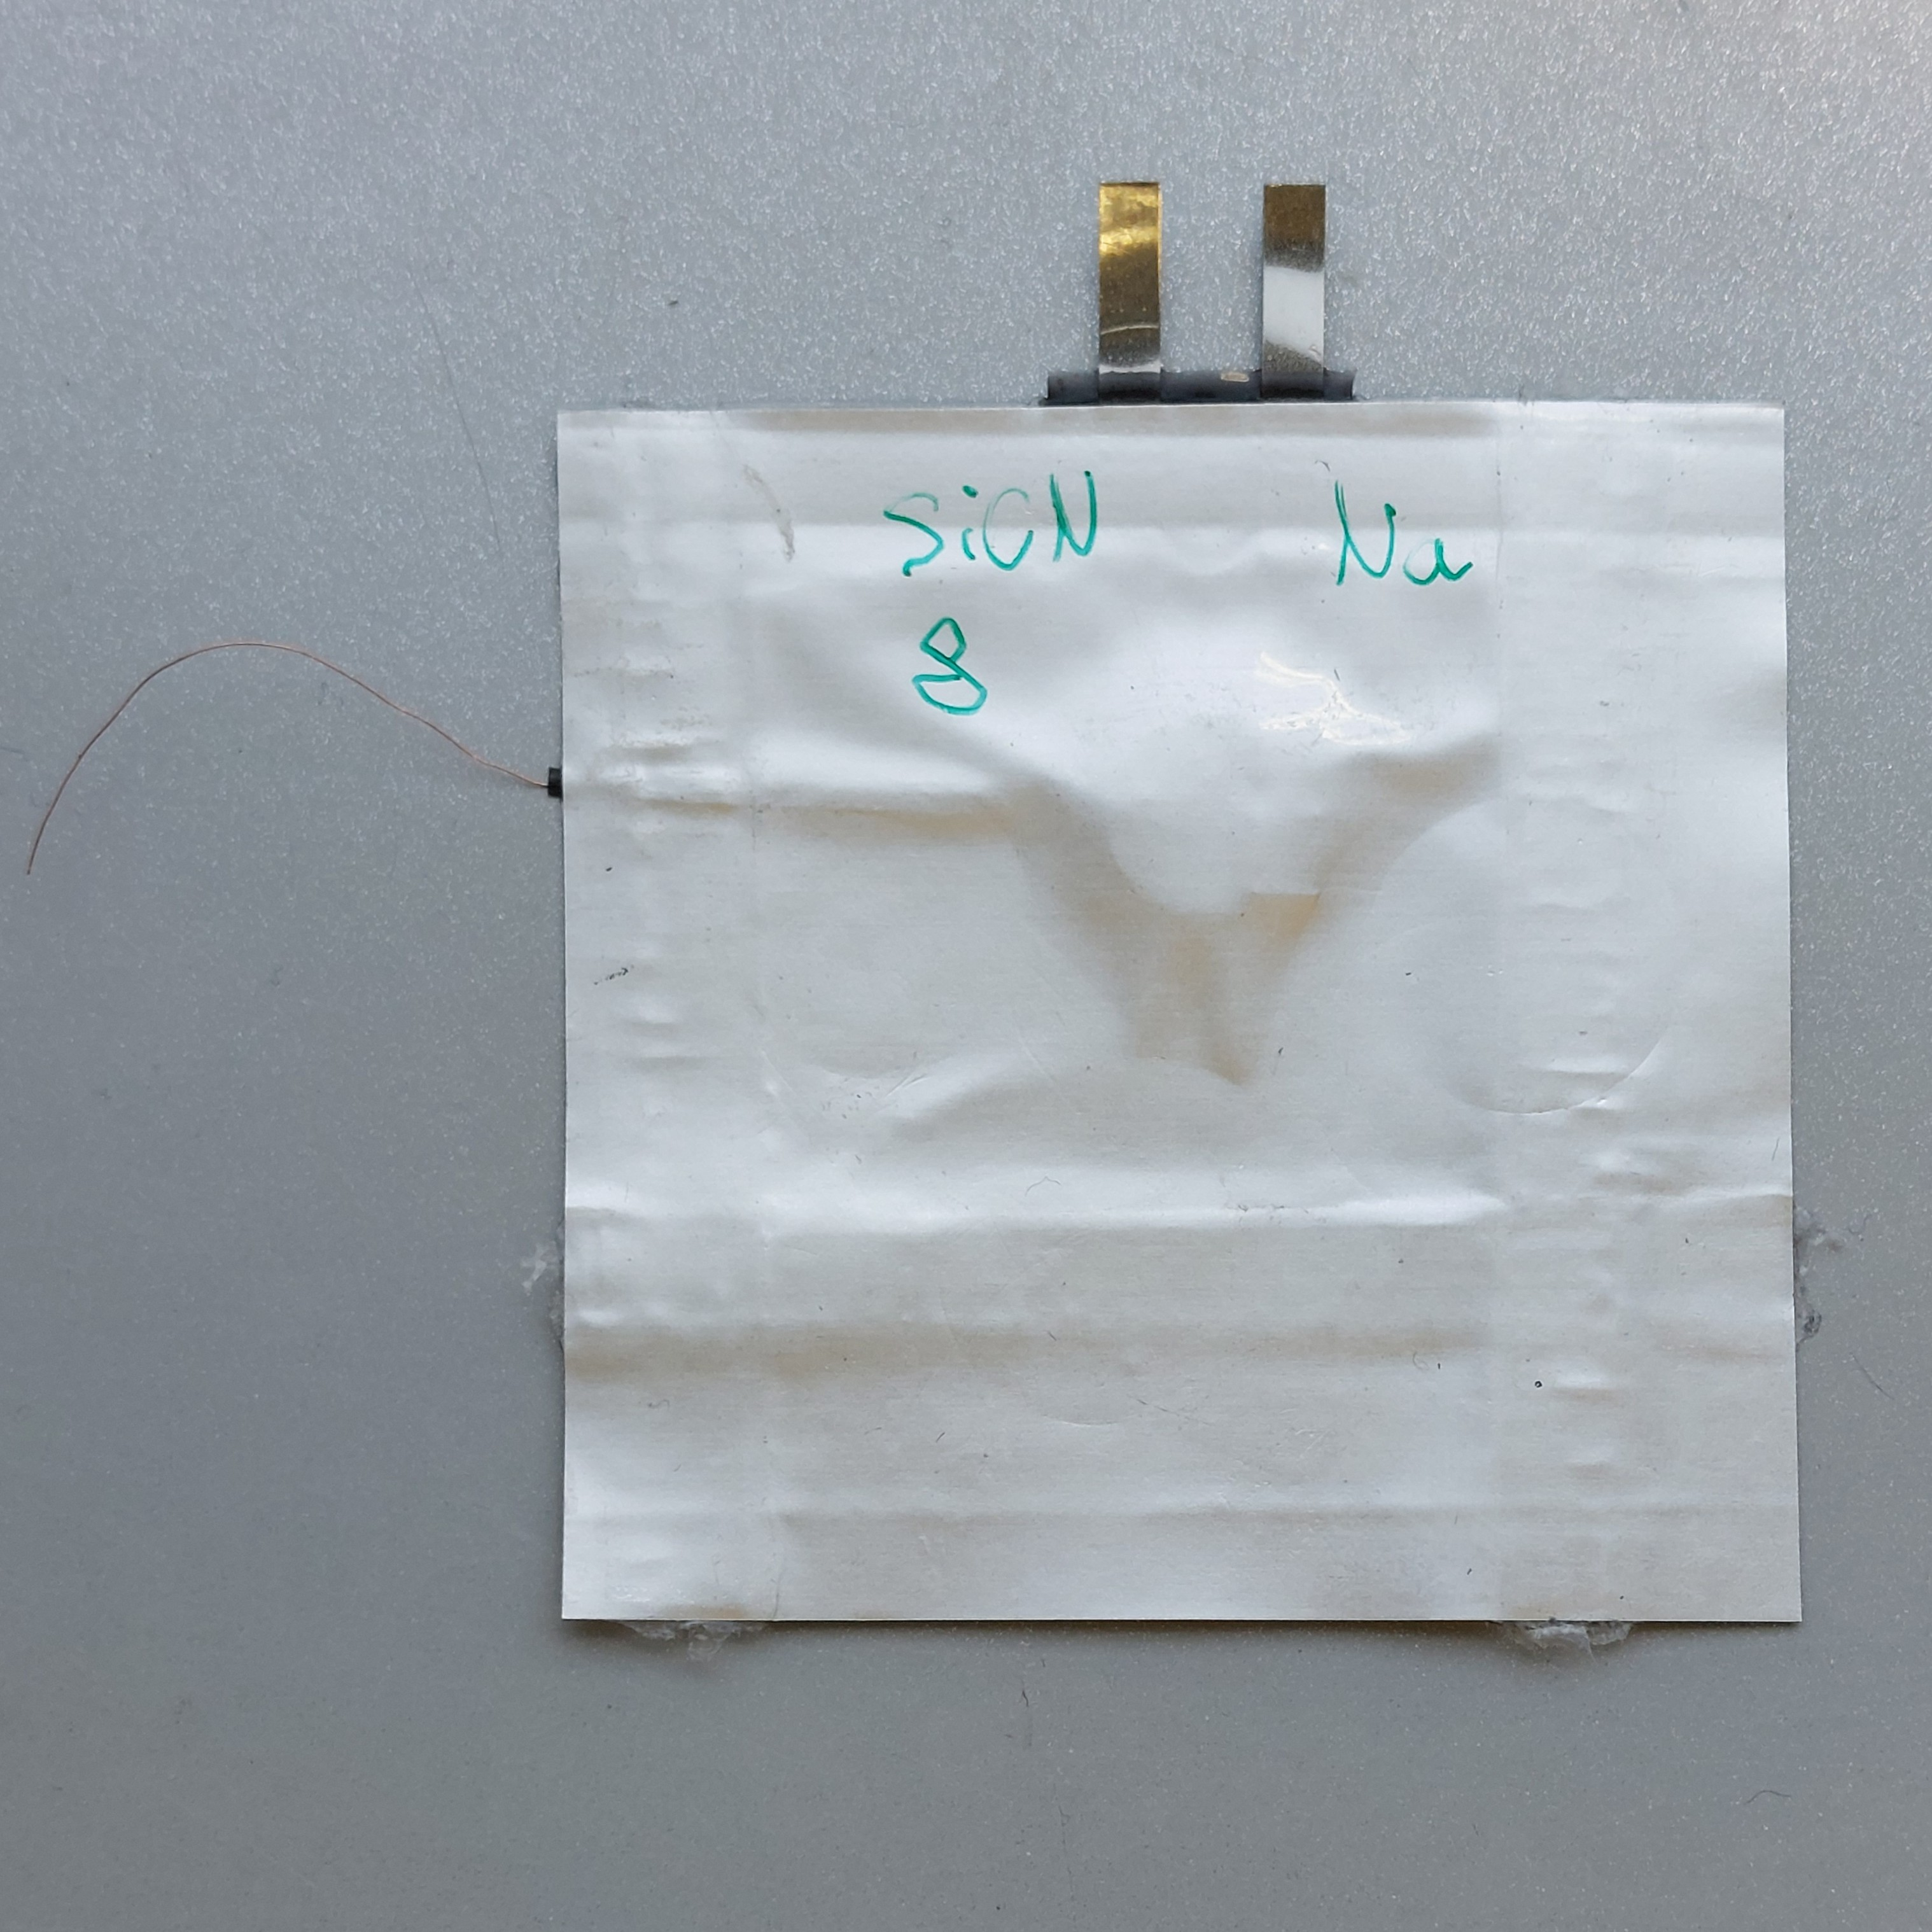
\includegraphics[width=0.38\textwidth]{figures/anodes/SiCN_final_pouch_3e.jpg}
    \caption{Three-electrode SiCN(O)/Na pouch cell with micro-reference electrode.
    Left: positioning of the microscopic reference electrode within the separator stack; right: completed three-electrode pouch cell used for operando DEIS measurements.}
    \label{fig:SiCNO_pouch}
\end{figure}

\subsection{DEIS measurement}

% The dynamic impedance measurements were performed using the automated DEIS platform described in the Methods chapters (\ref{ch:acquisition} - \ref{chap:estimation}).  
% In contrast to the earlier work reported in Chapters~\ref{chap:LTP} and \ref{chap:capacitor}, this version of the setup allowed fully automated long-term acquisitions, enabling uninterrupted measurements of multiple cycles even at low C-rates (C/10 or lower).
% However, the online high-frequency impedance computation was not yet implemented at this stage, so the frequency band of the excitation was limited to 5 decades.  
% All measurements were carried out in three-electrode pouch cells, with the working electrode connected to the potentiostat WE terminal, the counter electrode to CE, and the micro-reference electrode to RE.

\subsubsection{Multi-sine excitation}
For all chemistries, multi-sine excitations were generated using the Keysight TrueForm 33500-series waveform generator.  
The signals were constructed from non-intermodulating integer multiples of the fundamental frequency, with eight frequency points per decade and randomized phases to minimize the crest factor.  
Current and voltage responses were recorded using a PicoTech PicoScope 4000a at sampling rates between 5\,kHz and 50\,kHz depending on the upper frequency of the excitation band.  
The multisine amplitude was adjusted separately for each material to maintain linearity of the response and avoid saturating the potentiostat compliance limits.

\subsubsection{Applied drift and DEIS parameters for graphite}
Galvanostatic cycling was performed at three C-rates (C/5, 1C, and 2C), calculated from a theoretical graphite capacity of 11\,mAh.  
The potential limits were set to 0.8\,V and 0\,V vs.\ Li/Li$^+$.  
A multi-sine excitation containing frequency components from 0.01\,Hz to 1\,kHz was superimposed on the galvanostatic drift.  
Equal relative amplitudes were used across all sine components, and the phases were randomized to obtain the lowest crest factor.  
The perturbation amplitude was 40\,mA\textsubscript{pp} for the C/5 and 1C experiments.  
For the 2C experiment, the perturbation was reduced to 5\,mA\textsubscript{pp} to avoid non-linear distortion near the lower potential limit and to maintain the oscillation within the hardware compliance window.  
However, the impedance estimates at 2C were notably degraded by the reduced signal-to-noise ratio.

\subsubsection{Applied drift and DEIS parameters for SiCN(O)}
SiCN(O) electrodes were tested under galvanostatic cycling between 0\,V and 2.5\,V vs.\ Na/Na$^+$, using a C/10 current defined relative to the theoretical capacity reported in Reference \cite{derilReversibleSodiumPlating2023}.
Silicon carbonitride is an amorphous material; therefore, the maximum theoretical capacity cannot be calculated directly from its crystal structure as for typical inorganic materials.
A multi-sine excitation from 10\,mHz to 1\,kHz was used. 
A flat voltage amplitude of 80\,mV was applied at the generator; the resulting current perturbation depended on the potentiostat's selected current range and was monitored during acquisition.  
Voltage and current were sampled at 5\,kHz.

\subsubsection{Applied drift and DEIS parameters for metallic sodium}
Metallic sodium electrodes were cycled galvanostatically at 120\,\textmu A, corresponding to the C/10 rate adopted for the SiCN(O) experiments.  
The current was alternated between anodic and cathodic directions in 1\,h intervals to induce repeated sodium plating and stripping.  
The multi-sine excitation ranged from 0.02\,Hz to 20\,kHz, with relative amplitudes selected from prior DEIS measurements on an identical cell geometry.  
The signals were sampled at 50\,kHz to ensure adequate resolution of the highest-frequency components.

\subsubsection{Impedance estimation}
For all measurements, the instantanous impedance was estimated offline using the DMFA method.  
A symmetric Fermi-Dirac function with bandwidth between 0.01\,Hz and 0.02\,Hz (selected according to the lowest excitation frequency) and order $n=8$ was employed.  
Linear baselines were removed from both current and voltage signals prior to filtering to eliminate partially the DC offsets.  
The resulting time resolution of the impedance is the inverse of the bandwidth: 100 seconds (for graphite and SiCN(O)) or 50 seconds (for metallic sodium).

\section{Results and Discussion}

\subsection{Graphite}

\subsubsection{General behavior and formation}
Prior to the DEIS measurements, the graphite half-cells underwent a standard formation protocol followed by several galvanostatic cycles at 1C to ensure a stable SEI and reproducible electrochemical behavior. The DEIS results reported here correspond to galvanostatic cycling at different C-rates (C/5, 1C, and 2C) within the voltage window of 0--0.8\,V vs.\ Li/Li$^+$. The theoretical capacity of the electrodes (11\,mAh) was used to set the applied current.

\subsubsection{Instantaneous impednace at low currents}
Figure~\ref{fig:graphite_C5} shows the time-resolved impedance during a full C/5 cycle.
\begin{widefigure}[!h]
    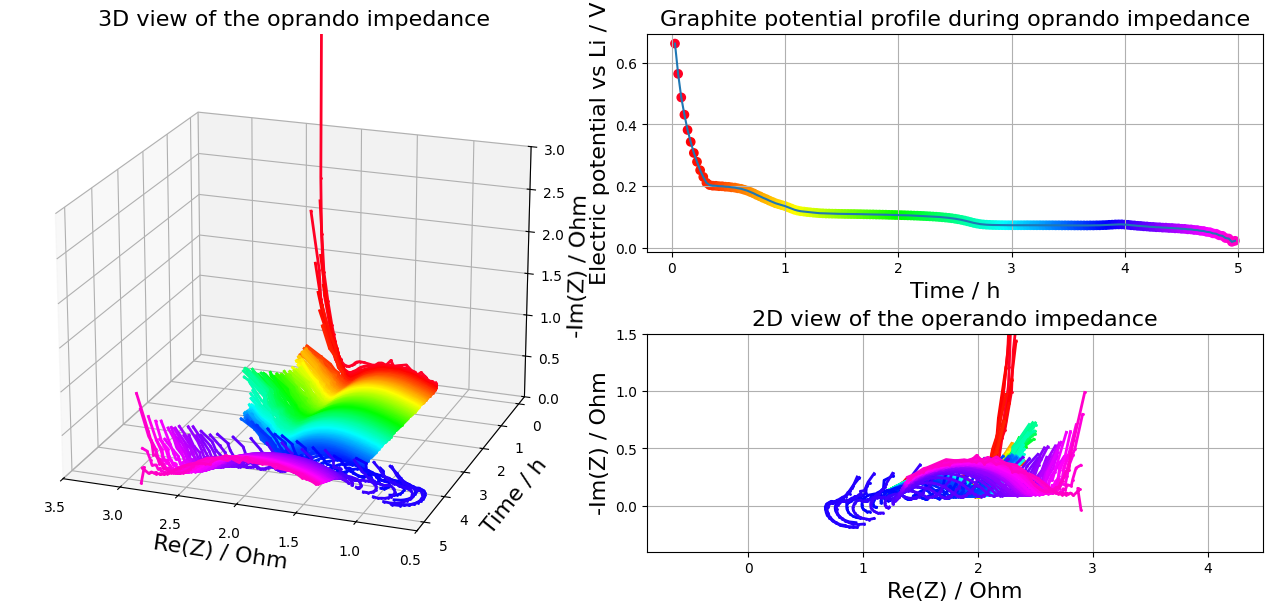
\includegraphics[width = 0.48\linewidth]{figures/anodes/graphite_reduction_C5.png}
    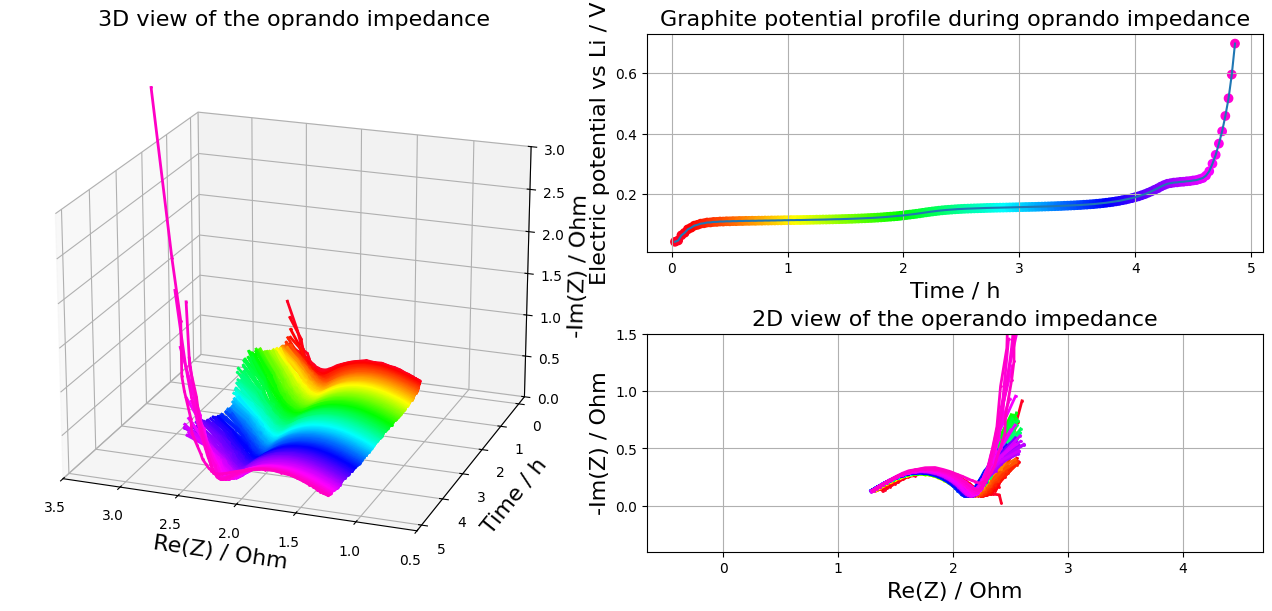
\includegraphics[width = 0.48\linewidth]{figures/anodes/graphite_oxidation_C5.png}
    \caption{Time-resolved impedance of graphite during a C/5 galvanostatic cycle.
    Dynamic impedance spectra acquired during lithiation (left) and delithiation (right), showing systematic evolution of low-frequency features across staging transitions. The first spectrum and lowest-frequency point were excluded.}
    \label{fig:graphite_C5}
\end{widefigure}

A clear evolution of the low-frequency diffusional tail is observed as the voltage crosses the characteristic graphite staging transitions.
This behavior is consistent for both lithiation and delithiation and parallels the trends previously reported for the LTP system in Chapter~\ref{chap:LTP}, suggesting that changes in intercalation-induced porosity, tortuosity, or solid-phase diffusion influence the instantaneous impedance.

Towards the end of lithiation, the impedance magnitude exhibits a sudden and transient reduction, after which it rapidly returns to its typical trajectory. Figure~\ref{fig:graphite_feature_zoom} highlights this local feature, and the instantaneous impedance spectrum at the minimum value is shown for clarity. 
\begin{figure}[!h]
    \centering
    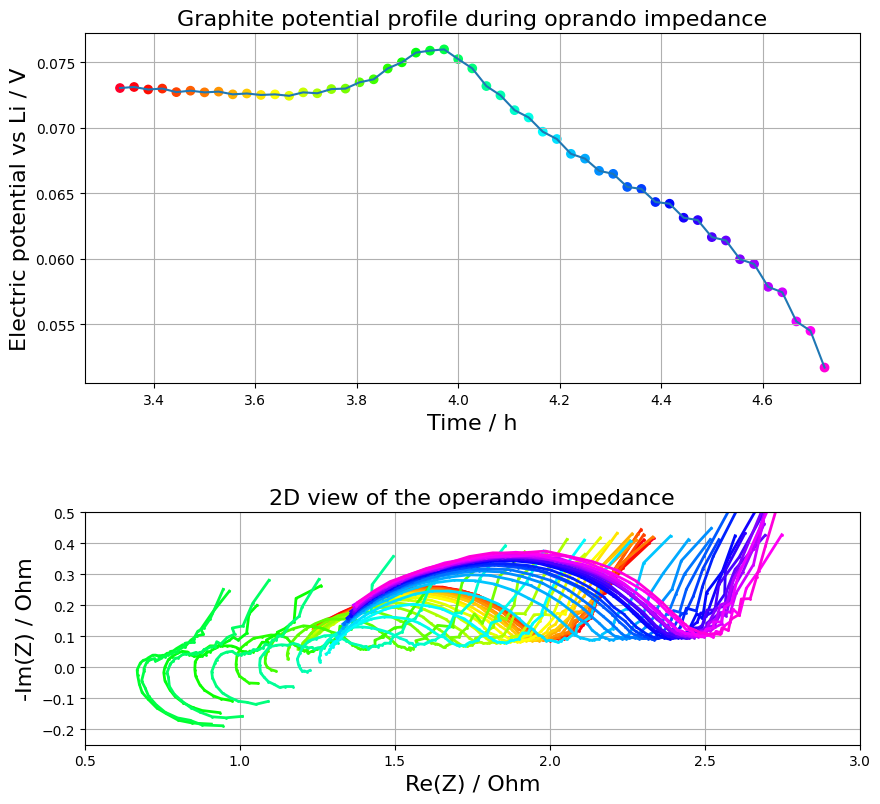
\includegraphics[width = 0.4\textwidth]{figures/anodes/graphite_feature_zoom.png}
    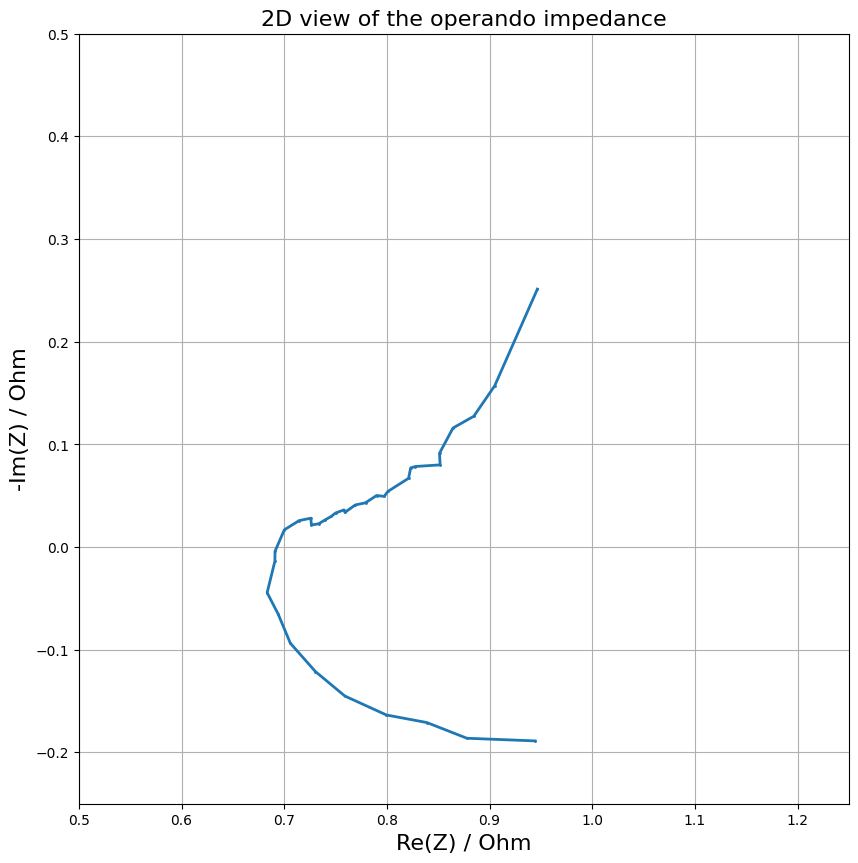
\includegraphics[width = 0.3\textwidth]{figures/anodes/graphite_single_impedance_feature.png}
    \caption{Localized transient impedance reduction during graphite lithiation.
    Left: zoomed view of impedance magnitude highlighting a brief drop near the end of lithiation; right: corresponding instantaneous impedance spectrum at the minimum, illustrating a temporary reduction in charge-transfer resistance.}
    \label{fig:graphite_feature_zoom}
\end{figure}
At this point the voltage simultaneously increases, implying a reduction in overpotential.
Importantly, the behavior is only observed under cathodic current, reinforcing the interpretation that it is not purely geometrical or diffusive in origin.
It is not clear weather the origin of such response is due to a structural rearrangment of the active material or parasitic reaction of the electrolyte or other contaminants in the cell actiated at that specific potential.

Unfortunalty, the signal-to-noise ratio worsens when the impedance becomes small relative to the perturbation amplitude, and this limits the precision of the estimation in this portion of the cycle.


\subsubsection{Instantaneous impednace at high currents}
At higher rates (1C and 2C), the behavior differs markedly. As shown in Figure~\ref{fig:graphite_1C}, neither the staging-related changes in the low-frequency region nor the transient impedance reduction are observed. At 1C, the system does not reach the third intercalation plateau due to substantial overpotential, and only approximately 70\,\% of the theoretical capacity is accessed. 
The high-frequency resistance and charge-transfer semicircle increase systematically with current rate, as is expected in regimes dominated by concentration polarisation and interfacial limitations.

\begin{widefigure}[!h]
    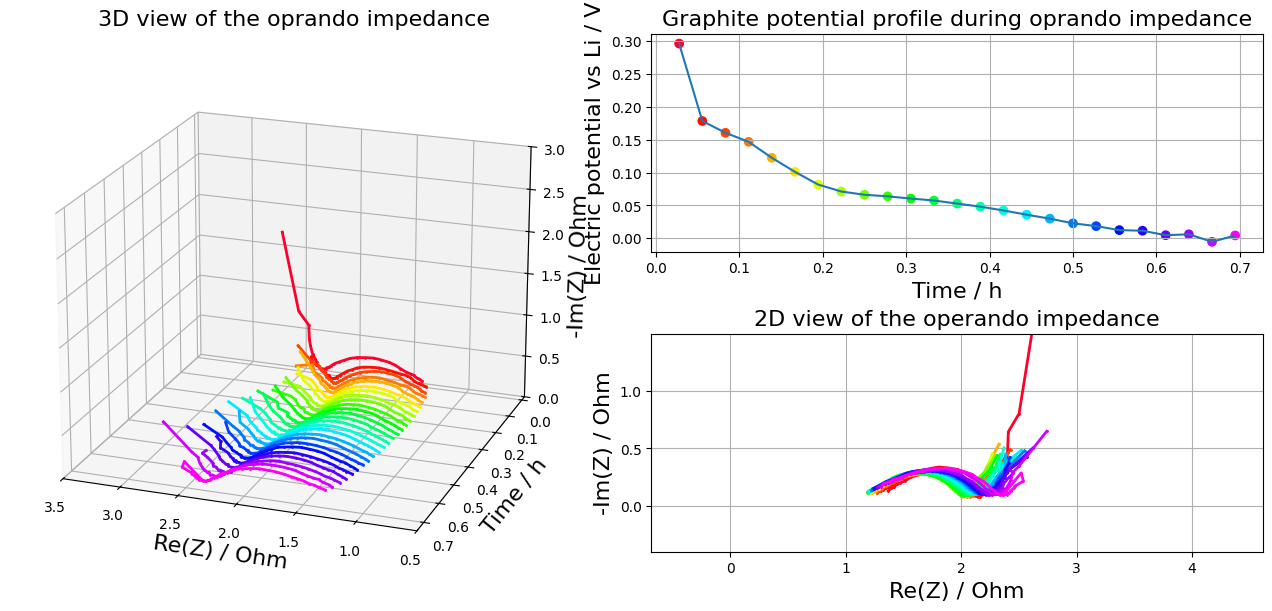
\includegraphics[width = 0.48\linewidth]{figures/anodes/graphite_reduction_1C.png}
    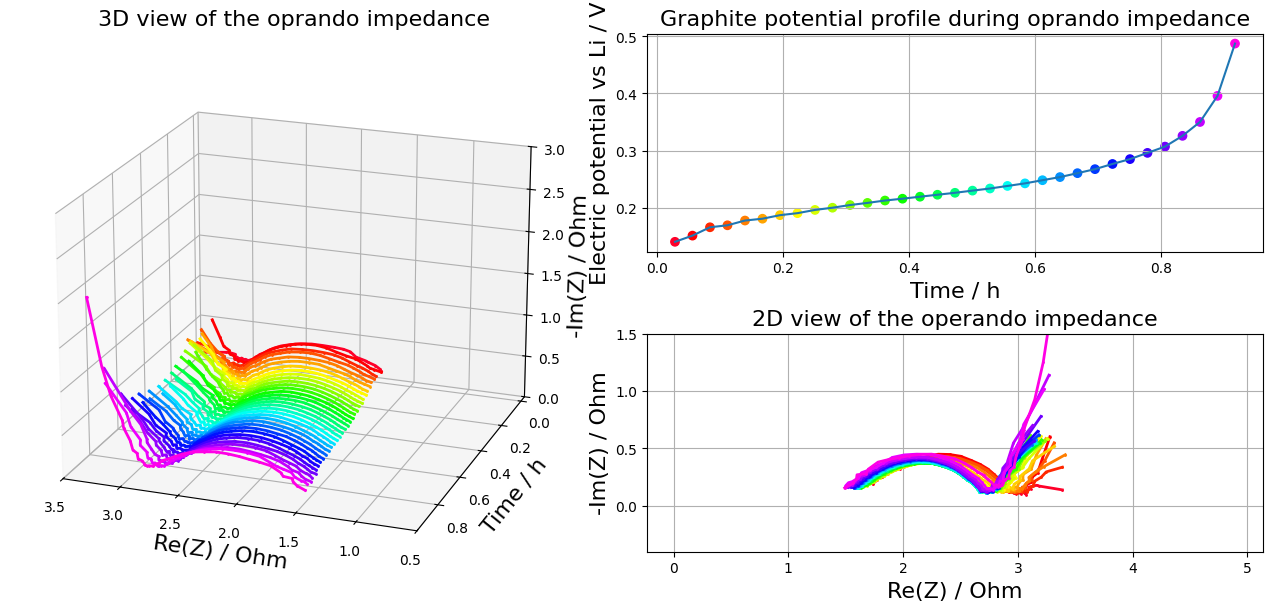
\includegraphics[width = 0.48\linewidth]{figures/anodes/graphite_oxidation_1C.png}
    \caption{Dynamic impedance during 1C galvanostatic lithiation/delithiation.}
    \label{fig:graphite_1C}
\end{widefigure}

\begin{widefigure}[!h]
    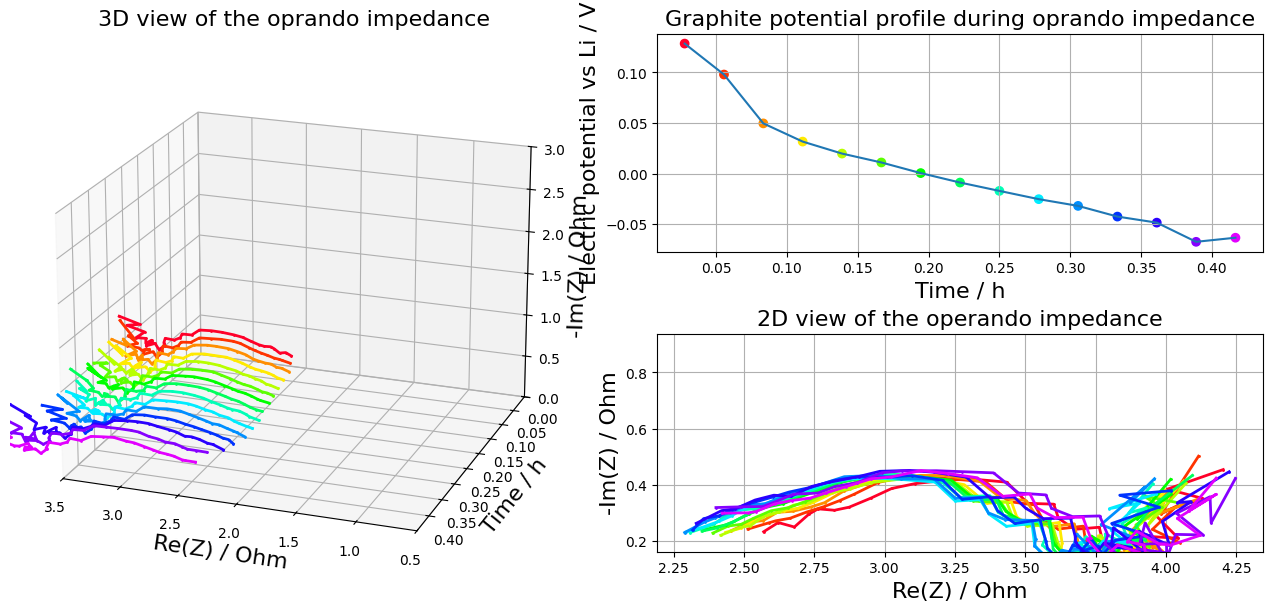
\includegraphics[width = 0.48\linewidth]{figures/anodes/graphite_reduction_2C.png}
    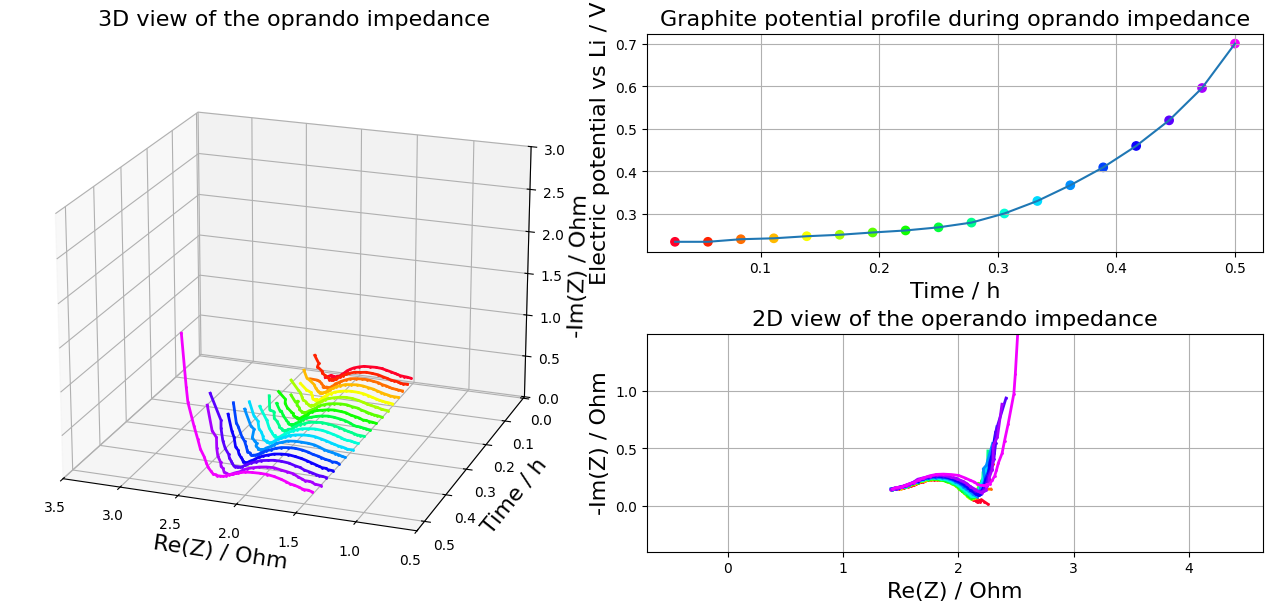
\includegraphics[width = 0.48\linewidth]{figures/anodes/graphite_oxidation_2C.png}
    \caption{Dynamic impedance during 2C galvanostatic lithiation/delithiation.}
    \label{fig:graphite_2C}
\end{widefigure}

To highlight the effect of current rate on the instantaneous impedance response, Figure \ref{fig:graphite impedance comparison} compares spectra at identical state of charge.

The increase in high-frequency resistance and in the semicircle diameter between 1C and 2C suggests an increas of Ohmic drop due to mass transport limitation and a variation fo the charge-transfer activation energy. 

At 2C the impedance becomes noisy despite reducing the excitation amplitude, indicating that the nonlinear operating point still limits the measurement quality.
The sources of low precision are poor signal-to-noise ratios and strong intermodulation produced by nonlinearity in mass-transport-controlled operational regimes.

\begin{widefigure}[!h]
    \centering
    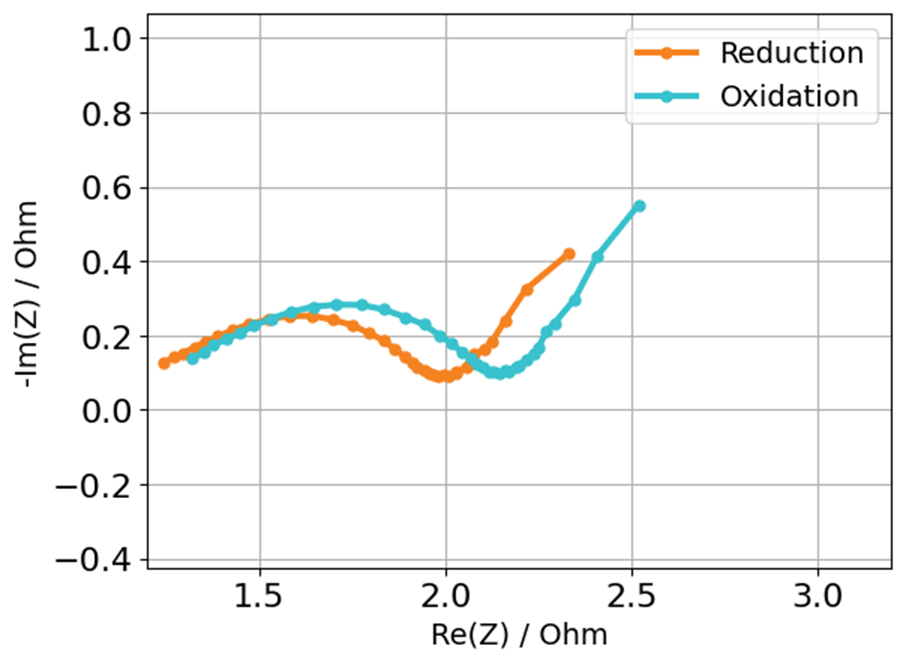
\includegraphics[width = 0.3\linewidth]{figures/anodes/image7.png}
    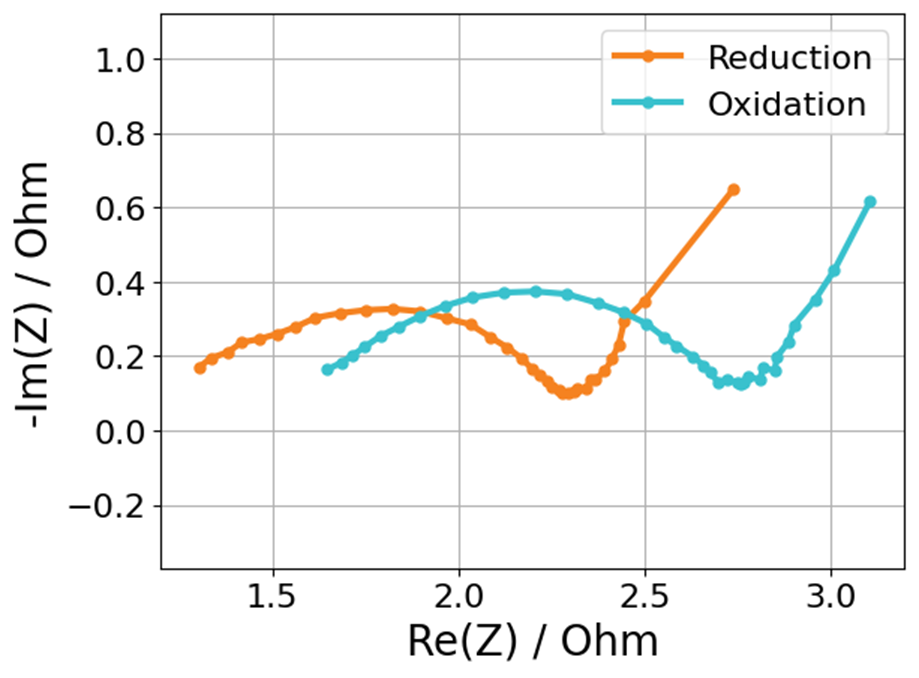
\includegraphics[width = 0.3\linewidth]{figures/anodes/image8.png}
    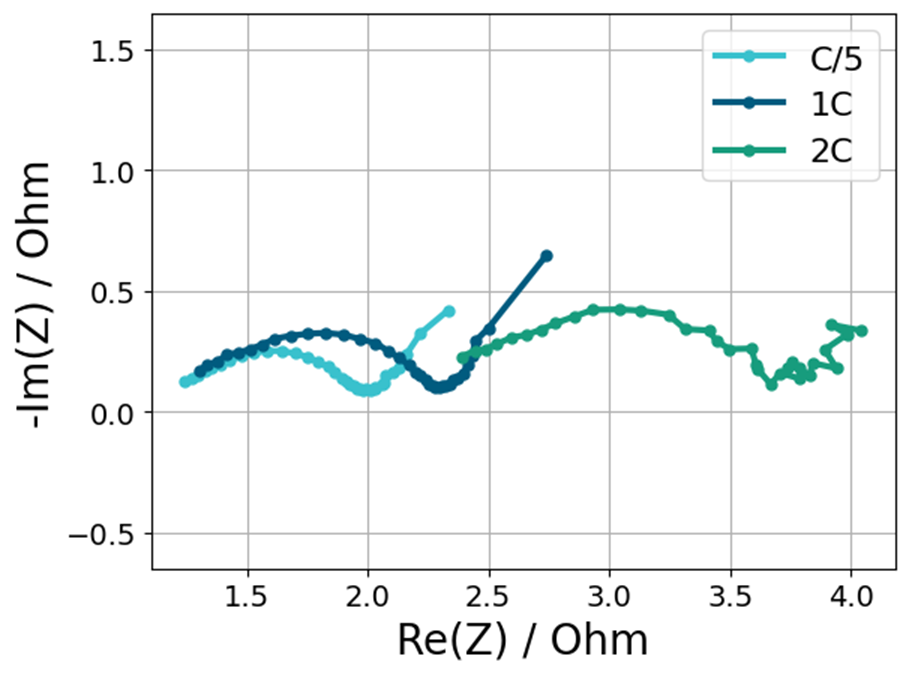
\includegraphics[width = 0.3\linewidth]{figures/anodes/image9.png}
    \caption{Effect of current rate on instantaneous graphite impedance.
    Comparison of impedance spectra at 50 \% state of charge for C/5, 1C, and 2C operation, illustrating the growth of high-frequency resistance and charge-transfer arcs with increasing current.}
    \label{fig:graphite impedance comparison}
\end{widefigure}

Attempts to reproduce the experiment with different graphite electrodes were not successful due to the difficulties in fabricating micro-reference electrodes via electrodeposition when SEI is also formed on the reference electrode tip. As a consequence, confirming whether the impedance transient stems from intrinsic electrochemistry or from electrode history effects remains an open question.

\subsection{SiCN(O)}

\subsubsection{First cycle: SEI formation}
The SiCN(O) electrodes were analyzed with dynamic impedance spectroscopy from pristine state, so the first cycle includes the SEI formation, as shown in Figure~\ref{fig:SiCN cell 36 first cycle}. 
In the 1.0--0.5\,V region, the impedance is large and then decreases sharply.%, consistent with the establishment of a passivation layer consuming Na$^+$. 
In the subsequent oxidation step, the impedance stabilizes, and in the following cycle (Figure \ref{fig:SiCN cell 36 second cycle}) the electrode behavior is distinct from the formation impedance.  
The accessible capacity is significantly lower than the nominal value used to calculate the nominal C-rate, confirming that the effective electrochemical capacity differs from the theoretical one.

\begin{widefigure}[!h]
    \centering
    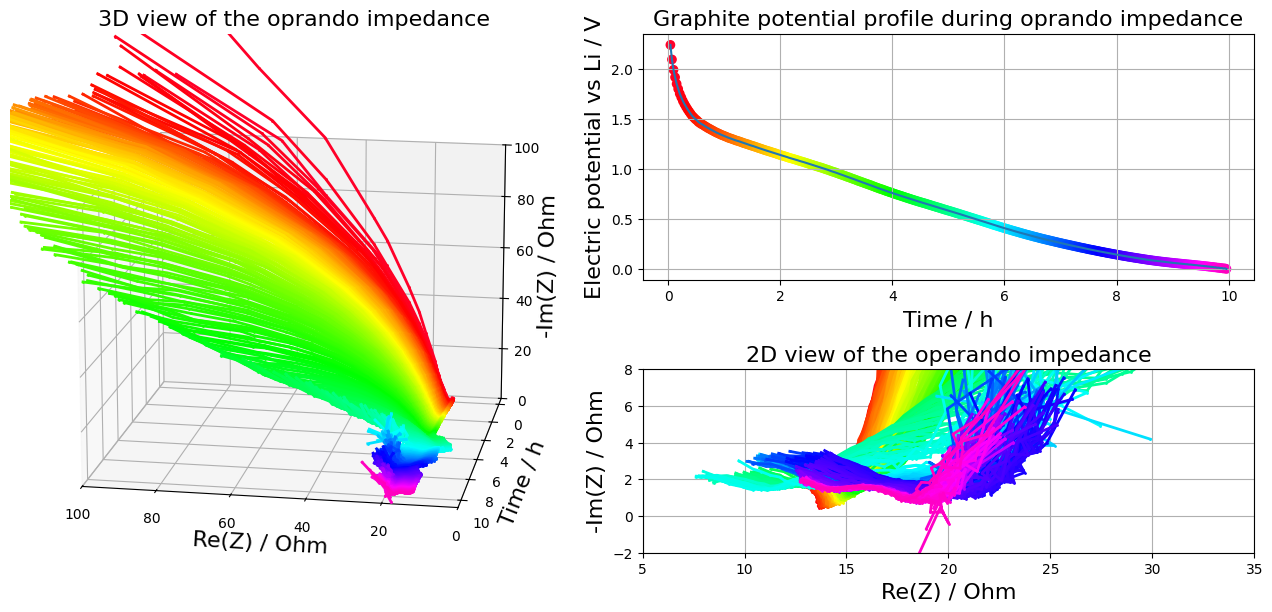
\includegraphics[width = 0.48\linewidth]{figures/anodes/SiCN_pouch36_1.png}
    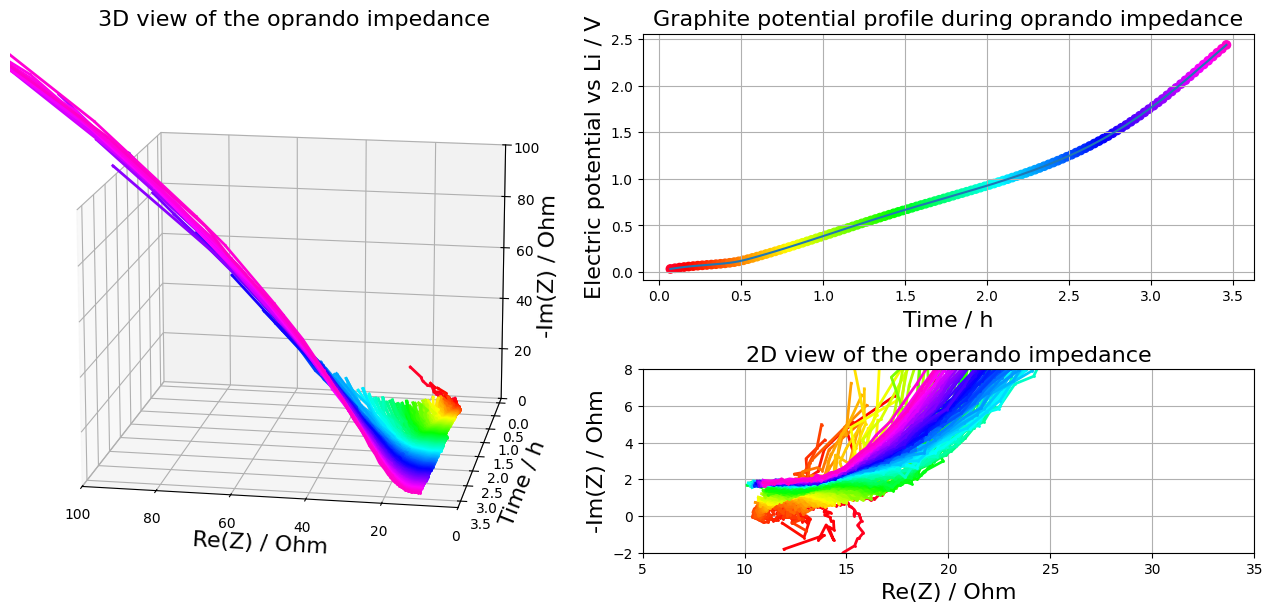
\includegraphics[width = 0.48\linewidth]{figures/anodes/SiCN_pouch36_2.png}
    \caption{First-cycle dynamic impedance of SiCN(O) during SEI formation.
    Time-resolved impedance during the initial sodiation/desodiation cycle at nominal C/10, showing high impedance in the 1.0-0.5 V region associated with SEI formation.}
    \label{fig:SiCN cell 36 first cycle}
\end{widefigure}

\begin{widefigure}[!h]
    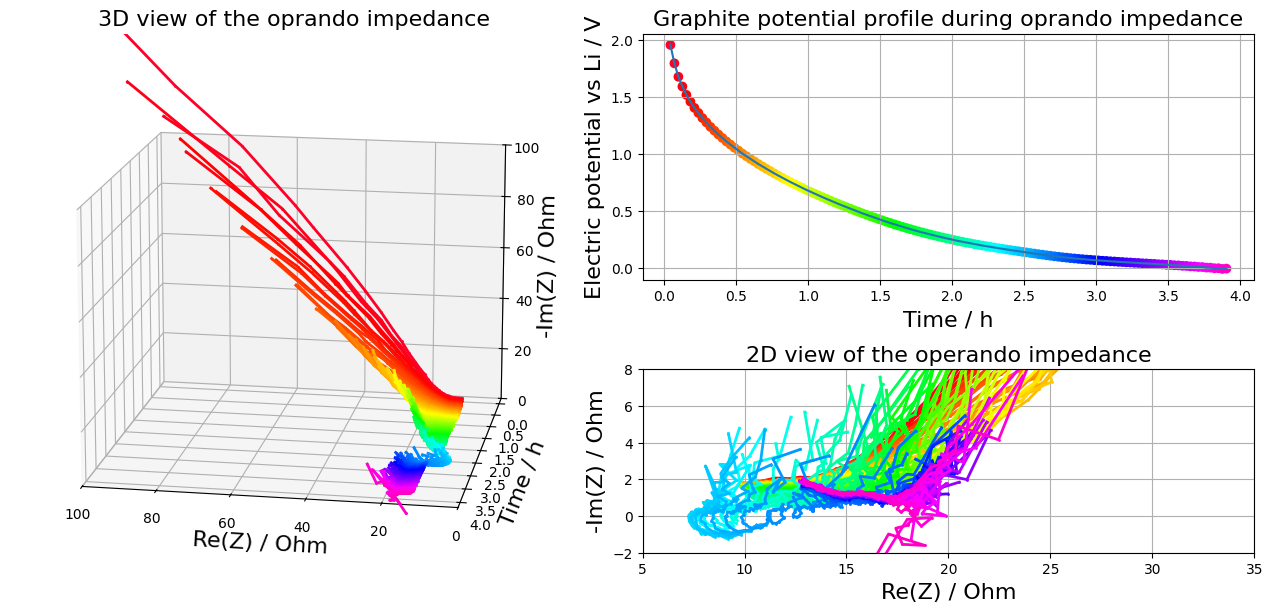
\includegraphics[width = 0.48\linewidth]{figures/anodes/SiCN_pouch36_3.png}
    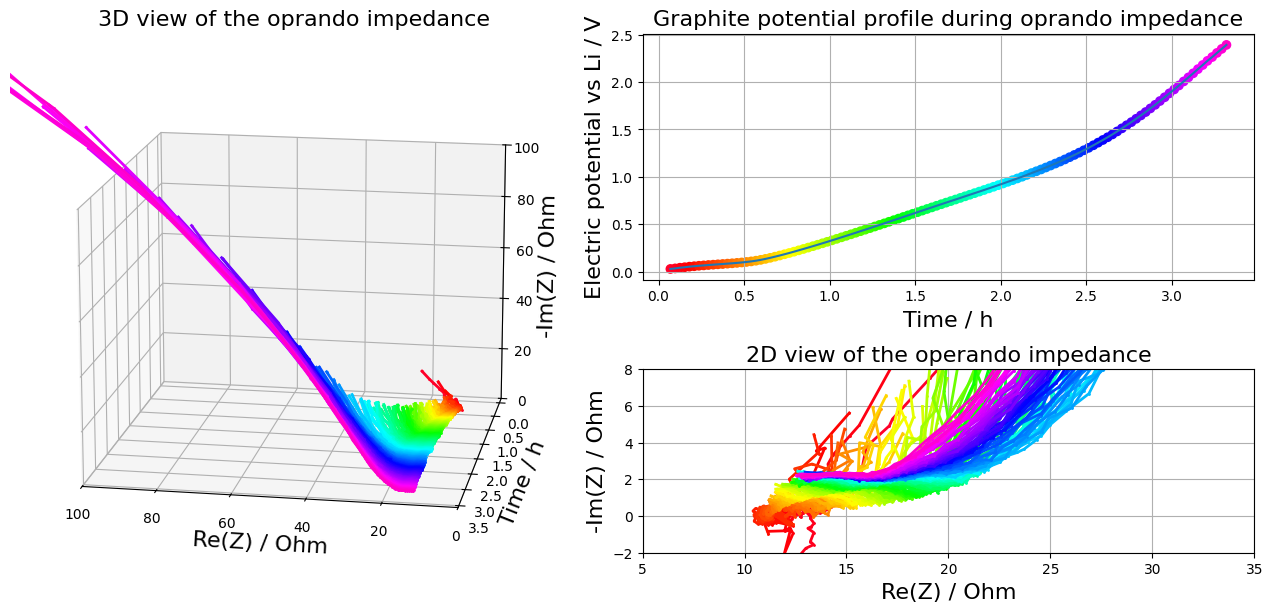
\includegraphics[width = 0.48\linewidth]{figures/anodes/SiCN_pouch36_4.png}
    \caption{Stabilized impedance response of SiCN(O) after formation.
    Dynamic impedance during the second cycle, demonstrating reduced and more stable impedance compared to the formation cycle.}
    \label{fig:SiCN cell 36 second cycle}
\end{widefigure}

\subsubsection{Transient impedance reduction}
A feature analogous to that observed for graphite appears in the second SiCN(O) cycle: a sudden reduction in impedance during the cathodic sweep. Figure~\ref{fig:SiCN_feature_zoom} illustrates this behavior and the associated instantaneous impedance spectrum. The spectral shape resembles that observed in graphite (Figure~\ref{fig:graphite_feature_zoom}), which suggests that the underlying mechanism might be similar, although not necessarily identical. Unlike in graphite, no simultaneous increase of the voltage is seen, which implies that the mechanism may be influenced by the specific surface chemistry of SiCN(O).

\begin{figure}[H]
    \centering
    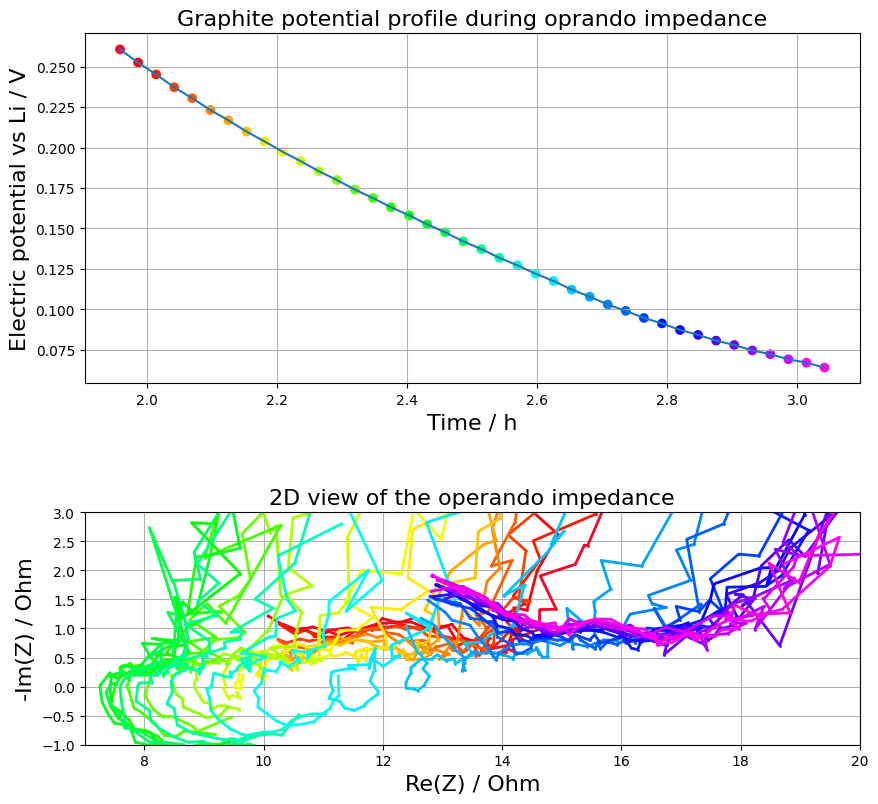
\includegraphics[width = 0.4\textwidth]{figures/anodes/SiCN_feature_zoom.png}
    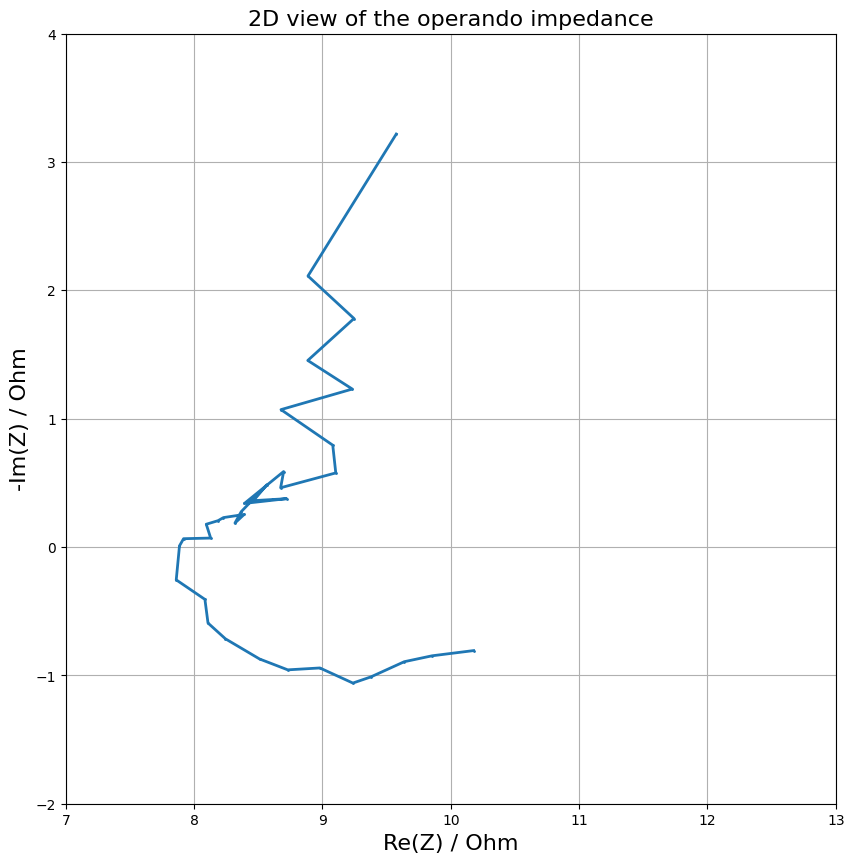
\includegraphics[width = 0.3\textwidth]{figures/anodes/SiCN_single_impedance_feature.png}
    \caption{Transient impedance reduction in SiCN(O) during sodiation.
    Zoomed impedance magnitude (left) and corresponding instantaneous spectrum (right) highlighting a brief reduction in impedance during the second cycle, qualitatively similar to the feature observed in graphite.}
    \label{fig:SiCN_feature_zoom}
\end{figure}

% \marginpar{
%     \centering
%     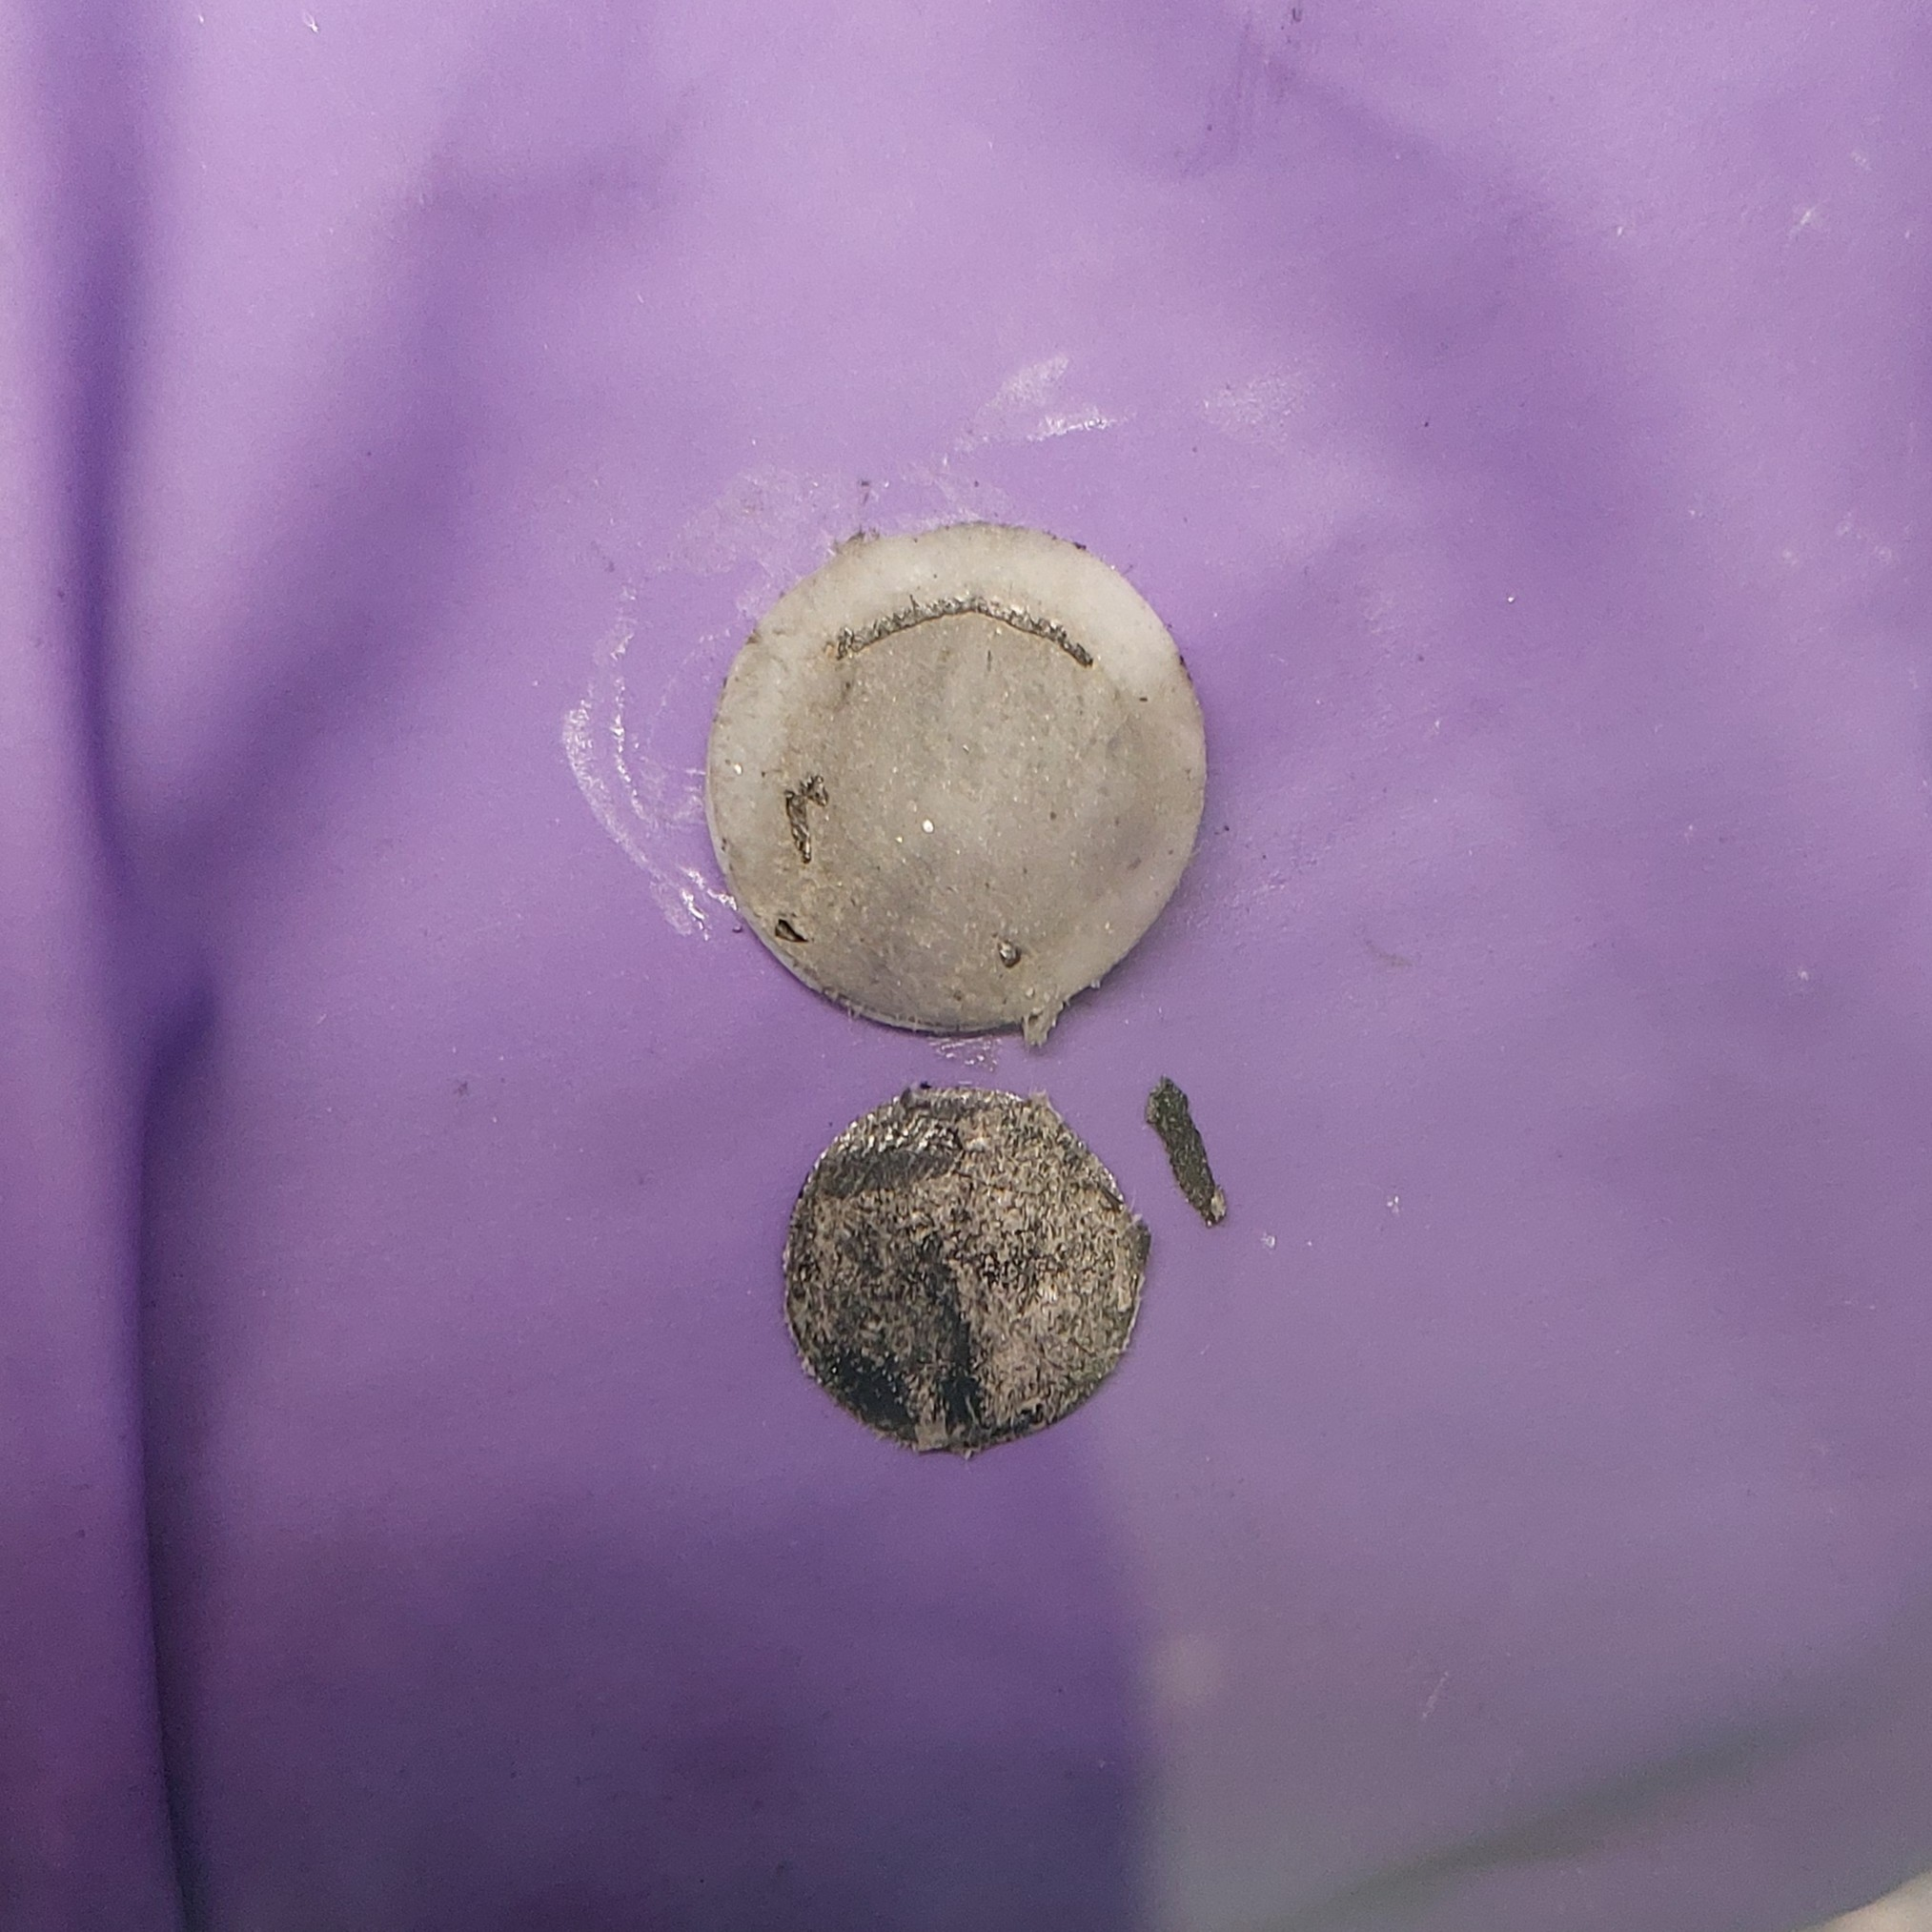
\includegraphics[width=0.9\marginparwidth]{figures/anodes/SiCN_post_mortem.jpg}
%     \captionof{figure}{Post-mortem evidence of sodium deposition on SiCN(O).
%     Optical image of the SiCN(O) electrode after cycling, showing metallic sodium deposits consistent with plating under the applied operating conditions.}
%     \label{fig:SiCN post mortem}
% }

% Because SiCN(O) is assumed to support reversible sodium metal deposition within microporosity (as previously proposed in the literature), one hypothesis is that metallic sodium nucleates within microcavities once a critical local overpotential is reached. Such a transition could transiently reduce the charge-transfer resistance. 

% Figure~\ref{fig:SiCN post mortem} shows a post-mortem image of the electrode with visible metallic sodium deposits, corroborating that plating does occur under the chosen operating conditions. However, this does not confirm that the impedance transient is caused by plating; it merely supports that plating is present.

A repetition of the experiment (Figures~\ref{fig:SiCN cell 39 first cycle}--\ref{fig:SiCN cell 39 third cycle}) revealed similar SEI formation behavior but did not show the transient impedance drop. This difference is plausibly attributable to variations in electrode porosity or local microstructure for the specific electrode.
Indeed Dr.-Ing. Melzi D'Eril observed lack of reproducibility of the "activation peak" for reversible electrodeposion \cite{derilReversibleSodiumPlating2023}.

\begin{widefigure}[!h]
    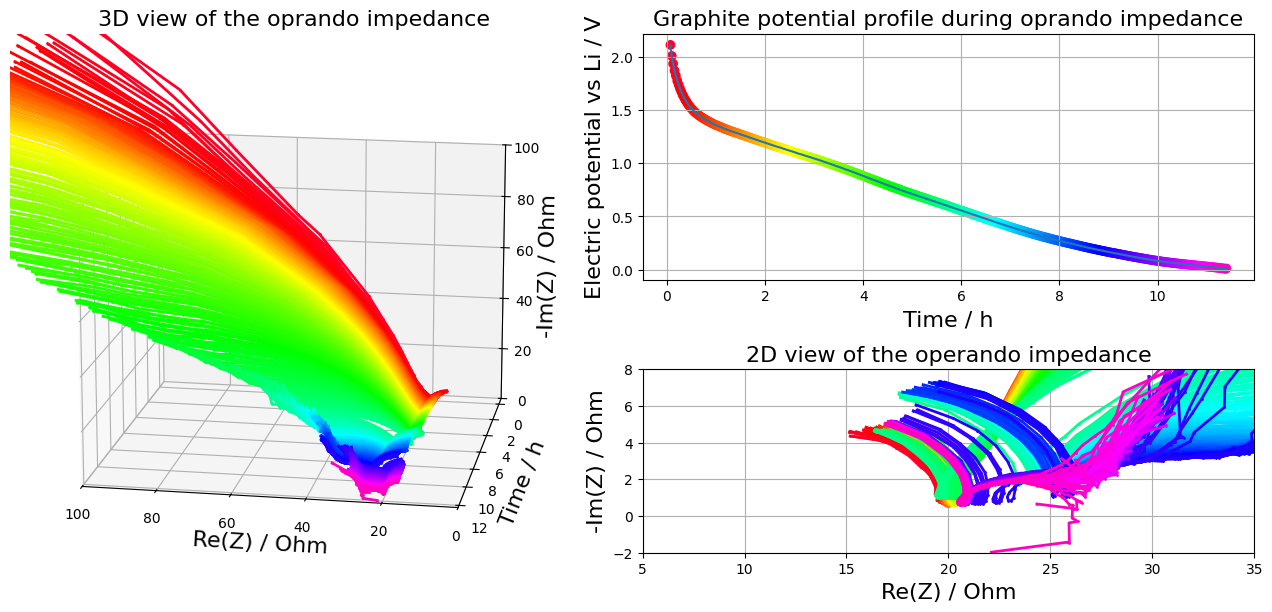
\includegraphics[width = 0.48\linewidth]{figures/anodes/SiCN_pouch39_1.png}
    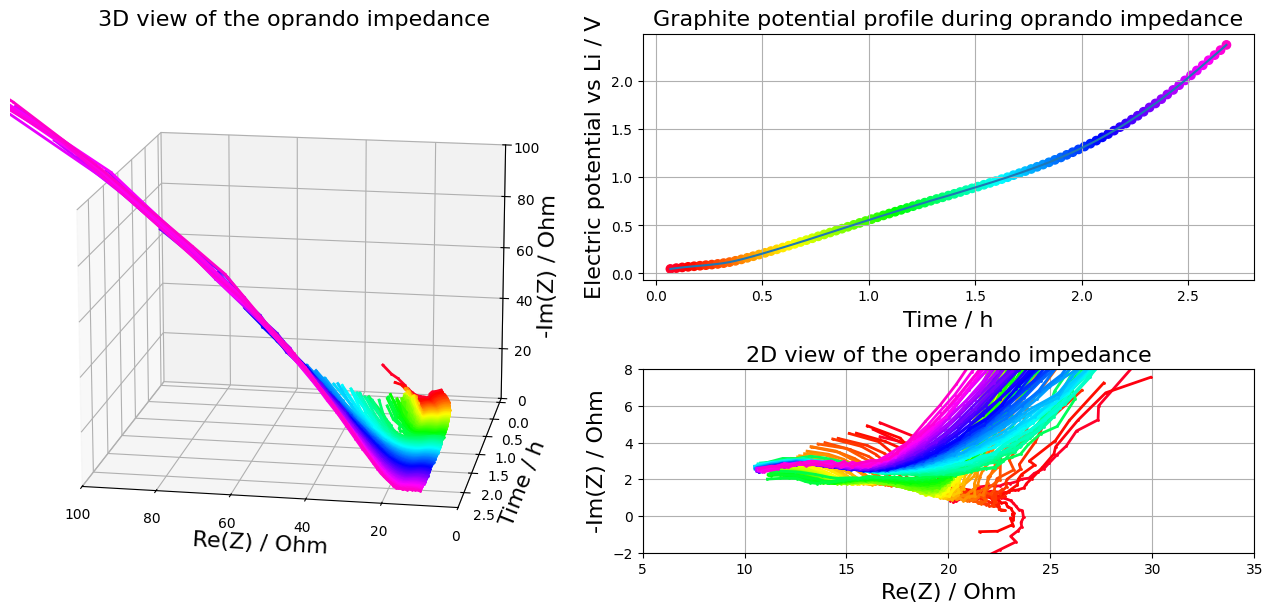
\includegraphics[width = 0.48\linewidth]{figures/anodes/SiCN_pouch39_2.png}
    \caption{First cycle of repeated SiCN(O) experiment.
    Dynamic impedance during initial sodiation/desodiation, showing SEI formation behavior comparable to the first cell.}
    \label{fig:SiCN cell 39 first cycle}
\end{widefigure}

\begin{widefigure}[!h]
    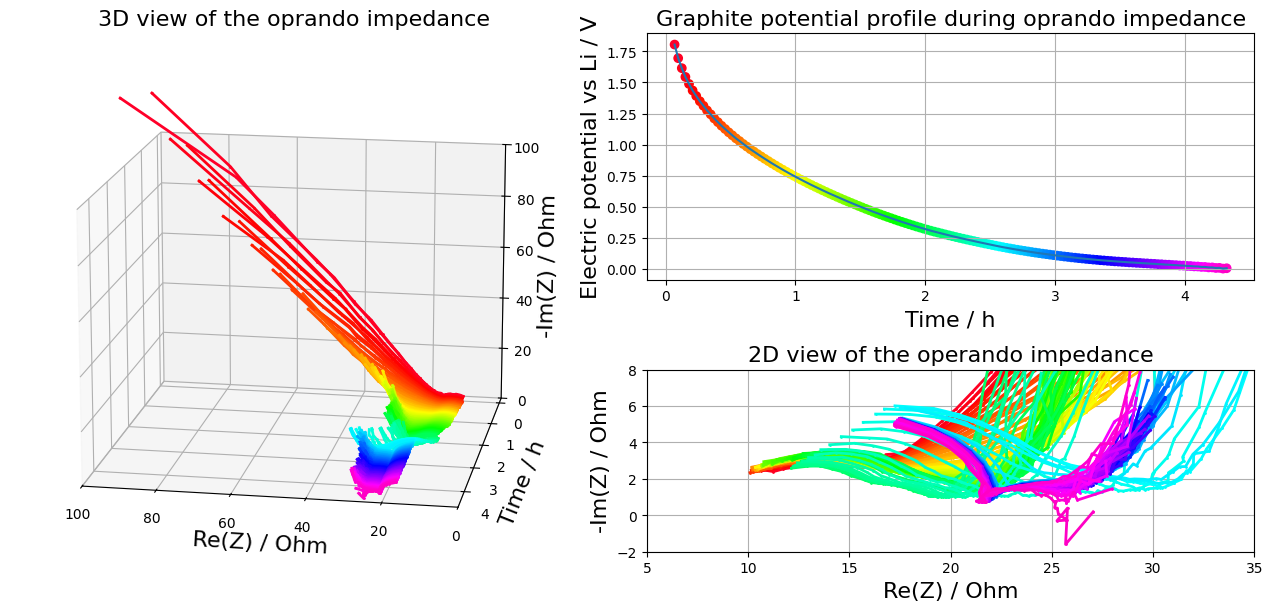
\includegraphics[width = 0.48\linewidth]{figures/anodes/SiCN_pouch39_3.png}
    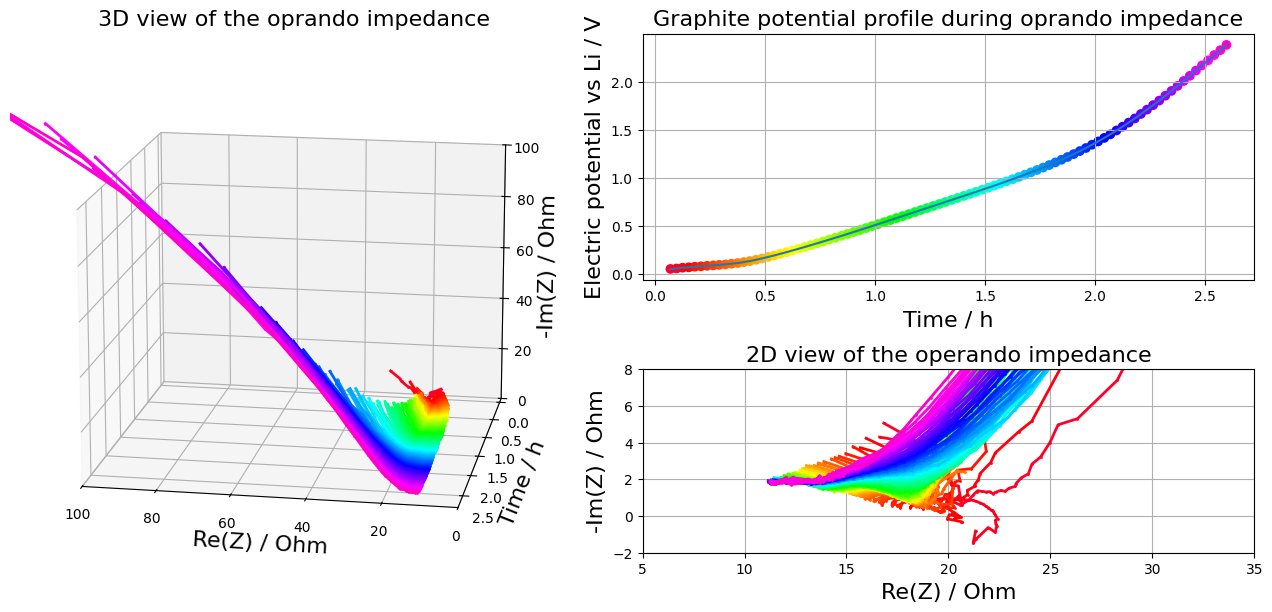
\includegraphics[width = 0.48\linewidth]{figures/anodes/SiCN_pouch39_4.png}
    \caption{Second cycle of repeated SiCN(O) experiment.
    Time-resolved impedance after formation, without appearance of a transient impedance drop.}
    \label{fig:SiCN cell 39 second cycle}
\end{widefigure}

\begin{widefigure}[!h]
    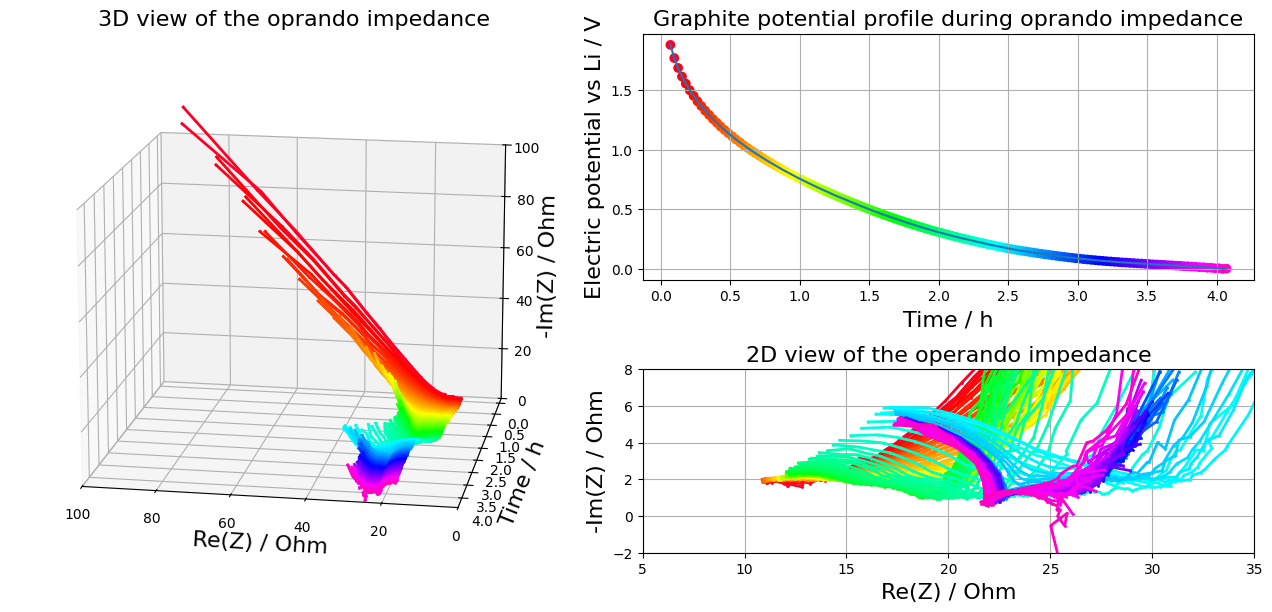
\includegraphics[width = 0.48\linewidth]{figures/anodes/SiCN_pouch39_5.png}
    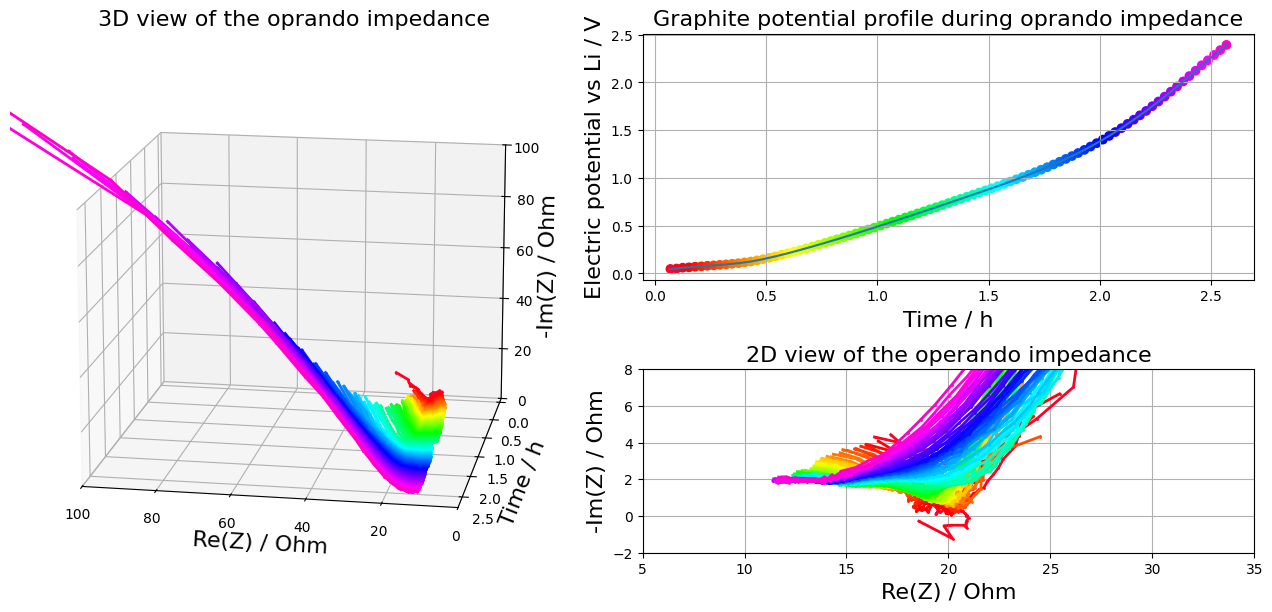
\includegraphics[width = 0.48\linewidth]{figures/anodes/SiCN_pouch39_6.png}
    \caption{Third cycle of repeated SiCN(O) experiment.
    Continued cycling showing stable impedance evolution and absence of transient features.}
    \label{fig:SiCN cell 39 third cycle}
\end{widefigure}

\subsubsection{Summary of SiCN(O) results}
Both SiCN(O) electrodes exhibit SEI formation followed by a stable impedance. 
Only one electrode displays a transient impedance reduction, making the effect non-reproducible with the present fabrication quality. 
Further studies with controlled porosity and improved reference-electrode reliability are required to evaluate whether the feature is mechanistically meaningful.

\subsection{Metallic Sodium}

\subsubsection{Plating behavior}
Metallic sodium plating and stripping were investigated to determine whether DEIS could detect specific mechanistic signatures associated with dendrite growth, SEI evolution, or nucleation processes. Prior to the DEIS cycle, a one-hour electrodeposition step at 120\,$\mu$A was performed to generate an SEI layer. After resting for several days, plating/stripping cycles were recorded.

During plating (Figure~\ref{fig:Na electrodeposition DEIS}), the impedance displays an inductive-like loop (positive imaginary part at intermediate frequencies), followed by a return toward lower resistance. 
\begin{figure}[h]
    \centering
    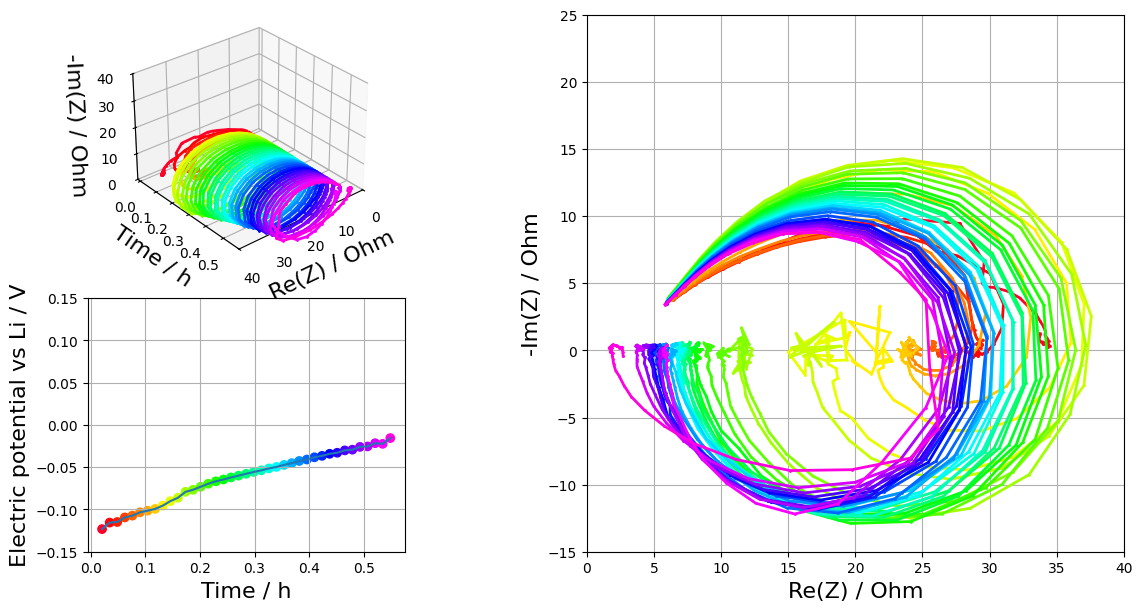
\includegraphics[width = \textwidth]{figures/anodes/sodium_pouch_1.png}
    \caption{Dynamic impedance during initial sodium plating.
    Time-resolved impedance spectra showing an inductive-like loop at intermediate frequencies during early sodium deposition, concurrent with decreasing overpotential.}
    \label{fig:Na electrodeposition DEIS}
\end{figure}
The overpotential decreases from approximately $-120$\,mV to $-10$\,mV, consistent with an increase in electrochemically active surface area during deposition.  
Such positive imaginary features have been reported in systems where a slow intermediate step precedes nucleation \cite{baiACImpedance1991, wuImpedanceDiskElectrode2009, spottiModelingElectrochemicalImpedance2026, brinkerInductiveLoops2024}. 
The specific mechanism on metallic electrodes coverd by SEI remains poorly documented, so the interpretation must remain tentative.

\subsubsection{Stripping behavior}
During stripping (Figure~\ref{fig:Na stripping DEIS}), the inductive loop rapidly disappears and the impedance shifts to a more conventional semicircle.
The overall magnitude increases with time, indicating a reduction in active surface area as the dendritic or mossy structures formed during plating dissolve. 
The absence of a diffusion tail across all cycles suggests that mass transport does not limit the reaction under the chosen conditions.

\begin{figure}[H]
    \centering
    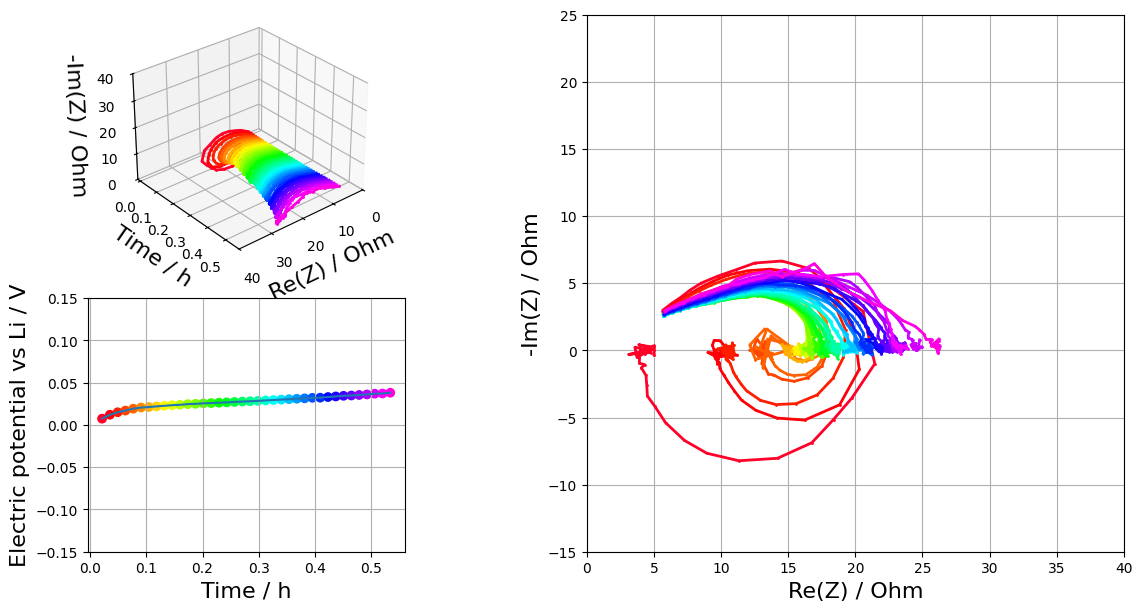
\includegraphics[width = \textwidth]{figures/anodes/sodium_pouch_2.png}
    \caption{Dynamic impedance during sodium stripping.
    Impedance evolution during anodic dissolution of sodium, characterized by disappearance of inductive features and increasing overall resistance.}
    \label{fig:Na stripping DEIS}
\end{figure}

\subsubsection{Repeated plating}
A second plating step (Figure~\ref{fig:Na second electrodeposition DEIS}) shows no inductive loop, despite maintaining similar overpotential ($\approx$50\,mV). 
\begin{figure}[H]
    \centering
    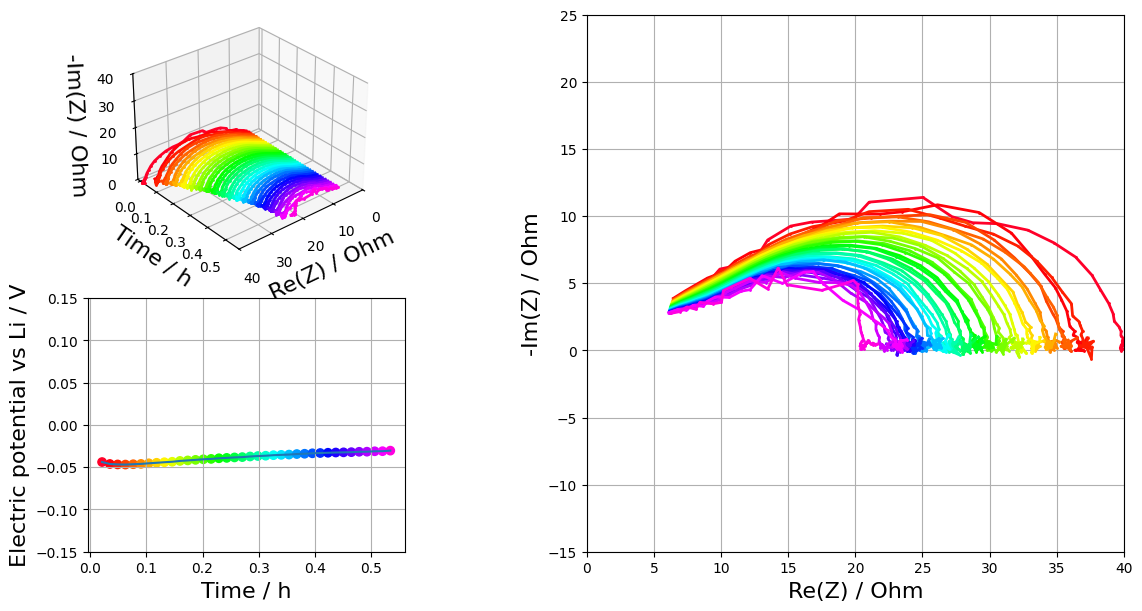
\includegraphics[width = \textwidth]{figures/anodes/sodium_pouch_3.png}
    \caption{Dynamic impedance during repeated sodium plating.
    Second electrodeposition cycle showing absence of the inductive loop observed during initial plating, indicating modified surface or SEI properties.}
    \label{fig:Na second electrodeposition DEIS}
\end{figure}
This suggests that the surface morphology or SEI structure no longer slow down the intermediate step that produced the positive imaginary part. 
Increasing impedance magnitude again correlates with increasing surface area during deposition.

\subsubsection{Summary of sodium results}
The sodium experiments highlight that DEIS is sensitive to morphology-dependent kinetic features during metal plating. The inductive-like behavior appears reproducibly in fresh sodium surfaces but disappears after the first stripping cycle, indicating that SEI and surface reconstruction strongly modify the interfacial dynamics. Access to higher frequencies would further clarify whether the origin of these features lies in nucleation kinetics, SEI viscoelasticity, or charge-transfer coupling.

\section{Major limitations and sources of uncertainty}

This work was conducted in parallel with the development of the DEIS software platform and experimental automation tools. 
As a consequence, several technical and methodological limitations affected data completeness, reproducibility, and interpretability. 
The most critical issues are summarised below.

\subsection*{Incomplete datasets and experimental continuity}

Because the measurement software and automated workflow were still under development, several datasets are incomplete. 
In some cases, full cycling histories are missing, and in others the acquisition was interrupted or partially corrupted. 
This limits the ability to reconstruct long-term trends in dynamic impedance or to compare electrodes across multiple, controlled operating conditions.

\subsection*{Micro-reference electrode fabrication and reproducibility}

A major source of uncertainty originates from the difficulty of fabricating reliable micro-reference electrodes.  
Despite extensive attempts, it was not possible to produce geometrically consistent references nor to ensure stable potentials over long experiments. 
As a result:

\begin{itemize}
    \item several measurements could not be repeated under identical electrochemical conditions;
    \item the assignment of certain impedance features,particularly those interpreted as transient plating-related signatures, could not be verified across multiple independent cells.
\end{itemize}

Given the extreme sensitivity of impedance to interfacial heterogeneity, reproducibility requires either identical electrode surfaces or a statistically meaningful number of repeats, neither of which was achievable with the present reference-electrode designs.

\subsection*{Deformation of the electrodes}

The micro-reference electrodes employed here had diameters comparable to those of the working electrodes (approximately $\sim50\,\mu$m). Even when used together with glass-fibre separators, their thickness is enough to altern the planarity of the electrode stack, that might be non-negligible for electrodes with small areas.
These geometric distortions may have influenced both the steady-state overpotential and the dynamic impedance response. Future implementations should consider thinner reference electrodes, meshes or grids structures to minimise localized pressure points.
% \begin{itemize}
%     \item thinner reference electrodes;
%     \item mesh or grid structures to minimise local pressure points;
%     \item reference electrodes based on intercalation compounds (e.g.\ LiFePO\textsubscript{4} or Na-based analogues), as commonly reported in the literature.
% \end{itemize}

% Such solutions would reduce mechanical intrusion and stabilise the reference potential.

\subsection*{Pouch-cell sealing}

Certain pouch cells exhibited uneffective sealing, which was only discovered long after the experiments.  
In at least one case, part of the pouch was open, allowing air ingress. Oxygen and moisture contamination are well known to trigger parasitic reactions with alkali metals and to alter SEI composition\cite{KAWAMURA2006547}, thereby affecting both voltage profiles and impedance.

Given the high reactivity of lithium and sodium systems, even small leaks can significantly distort the interfacial kinetics and compromise the interpretation of dynamic impedance features.

% \subsection*{Electrode-to-electrode variability}

% The SiCN(O) electrodes used in this study were characterized by meaningful microstructural variations related to their manufacturing process (porosity, binder distribution, carbon domain connectivity). Since impedance is intrinsically sensitive to surface condition and morphology, these variations produced:

% \begin{itemize}
%     \item significant differences in impedance magnitude between nominally identical cells;
%     \item non-reproducible appearance or disappearance of transient impedance features;
%     \item uncertainty in attributing observed behavior to fundamental electrochemistry rather than electrode heterogeneity.
% \end{itemize}

% Improved fabrication control or statistically larger sample sets are required to draw conclusive mechanistic interpretations.

% \subsection{Summary of limitations}

% In summary, the main constraints of this work are associated with reference-electrode reliability, mechanical perturbation by thick wires, occasional pouch-cell leaks, electrode variability, and software-development-related data omissions. While none of these invalidate the qualitative observations reported in the Results section, they restrict the strength of the mechanistic claims that can be made. Future work equipped with the latest automated DEIS instrumentation, high-quality reference electrodes, and strictly controlled cell assembly protocols is expected to overcome these limitations.

\section{Chapter summary and perspectives}

This chapter demonstrates that dynamic electrochemical impedance spectroscopy can be successfully imployed to probe electrochemical processes \emph{in situ} under operating conditions. Specifically, I performed experimetns in half-cells configuration of different negative electrode for lithium and sodium ion batteries.

Instantanous impednace of graphite electrode, isolate trhough the use of a reference electrode, reflected the staging transitions analogous to those observed for LTP in Chapter~\ref{chap:LTP} and revealed that at C/5 a reproducible transient impedance reduction appeared near the end of lithiation. 
Despite the origin is not clear, it shows how DEIS can be effective to probe processes characteristic of operative conditions.
Critically, this impedance feature appeared only during cathodic galvanostatic techniques and disappeared at higher rates (1C, 2C).

For SiCN(O) electrodes, DEIS successfully captured SEI formation during the first cycle, evidenced by high and evolving impedance in the 1.0--0.5\,V region. 
In subsequent cycles, one electrode exhibited a transient impedance reduction qualitatively similar to graphite, while the second did not. 
The difference of impedance between samples indicates sensitivity to electrode microstructure.
For this experiment an electroplated micro-reference electrode of metallic sodium was successfully reproduced multiple times and demonstrated potential stability for up to dozens of hours, enabling the completion of multiple cycles of galvanostatic techniques even at low C-rates.
This is remarkable for the fact that such type of stable electrodes are not yet reported in the literature.

Symmetric sodium cell measurements revealed distinctive signatures of metal plating and stripping dynamics. During initial plating, a positive imaginary impedance component (inductive-like loop) appeared at intermediate frequencies while overpotential decreased from $-120$\,mV to $-10$\,mV, suggesting nucleation kinetics or SEI-mediated surface reconstruction as rate-limiting. This feature did not reappear in subsequent plating, indicating irreversible surface morphology changes. During stripping, impedance evolved toward conventional semicircle behavior with increasing magnitude, consistent with dissolution of high-surface-area dendritic structures.

This chapter lays the foundation to fill the gap between the electrode level characterization   (Chapters~\ref{chap:LTP} and \ref{chap:capacitor}) and the monitoring of aging of commercial full cells (Chapter~\ref{chap:coins}). 

The inability to fully reproduce certain features highlights a fundamental challenge: electrochemical behavior is strongly influenced by preparation history, surface heterogeneity, and local microstructure. DEIS reveals this variability with high sensitivity, underscoring the need for both improved fabrication protocols and statistical approaches to impedance analysis.

Despite significant methodological challenges, particularly micro-reference electrode fabrication for lithium, the measurements reveal qualitatively consistent features that provide valuable mechanistic insights and motivate targeted future investigations.
This work demonstrates the capability of DEIS to resolve electrode-specific processes in three-electrode pouch cells under different operating conditions. 
The characteristic impedance features observed in negative electrodes of two different chemistries suggests an underlying physical origin worthy of a future systematic investigation.